\documentclass[12pt]{article}
\usepackage[utf8]{inputenc}
\usepackage{mdframed}
\usepackage{minted}
\usepackage{fullpage,enumitem,amsmath,amssymb,graphicx,centernot,amssymb, xcolor, float, tabularx, algorithmic}
\usepackage[ruled,vlined,commentsnumbered,titlenotnumbered]{algorithm2e}
\usepackage[breakable]{tcolorbox}
\usepackage{tikz, url}
\usepackage[usenames,dvipsnames]{color} 
\usetikzlibrary{calc, backgrounds}
\tikzset{vertex/.style={draw=none, line width = 2.4pt, fill, inner sep = .09cm, circle}}
\tikzset{edge/.style={very thick, gray, line cap=round}}

\begin{document}
\begin{center}
      \Large\textbf{CS161 Final Study Guide}\\
      \large\textit{Summer 2022}
\end{center}
\tableofcontents

\section{Divide and Conquer}

\subsection*{Big-O definitions}
Big-O notation gives an upper bound on a function. We say $T(n)$ is $O(f(n))$ when as $n$ gets big, $f(n)$ grows at least as quickly as $T(n)$. Formally, we say

$$
T(n)=O(f(n)) \Longleftrightarrow \exists c, n_{0}>0 \text { s.t. } \forall n \geq n_{0}, 0 \leq T(n) \leq c \cdot f(n)
$$
Big-Omega notation gives a lower bound on a function. We say $T(n)$ is $\Omega(f(n))$ when as $n$ gets big, $f(n)$ grows at least as slowly as $T(n)$. Formally, we say
$$
T(n)=\Omega(f(n)) \Longleftrightarrow \exists c, n_{0}>0 \text { s.t. } \forall n \geq n_{0}, 0 \leq c \cdot f(n) \leq T(n)
$$
\subsection*{Big-O proofs}
If $f(n)=O(g(n))$, then $f(n)^{2}=O\left(g(n)^{2}\right)$. (Note: $f(n)^{2}$ is the square of $f(n)$, not $\left.f\left(n^{2}\right)\right)$
\begin{tcolorbox}
This is true. Because $f(n)=O(g(n))$, there exist $c, n_{0}$ such that for all $n \geq n_{0}, f(n) \leq$ $c \cdot g(n)$. Now square both sides of this inequality. Because $x^{2}$ is a strictly increasing function, we have:$$f(n)^{2} \leq c^{2} \cdot g(n)^{2}
$$
But now take $c^{\prime}=c^{2}$ and $n_{0}^{\prime}=n_{0}$, and we see that for all $n>n_{0}^{\prime}$, $f(n)^{2} \leq c^{\prime} \cdot g(n)^{2}$. Therefore $f(n)^{2}=O\left(g(n)^{2}\right)$.
\end{tcolorbox}
Show that if $f(n)=O(g(n))$, then $2^{f(n)}=O\left(2^{g(n)}\right)$ is false. 
\begin{tcolorbox} 
Here is a simple counterexample: Let $f(n)=2 n, g(n)=n$. We need to show that $2 n=O(n)$, and $2^{2 n}$ is not $O\left(2^{n}\right)$. Fortunately, neither is too hard to show:
\begin{itemize}
\item $2 n=O(n):$ Choose $n_{0}=1, c=2$. Then for all $n \geq n_{0}$, we see (pretty trivially) that $2 n \leq 2 \cdot n$.
\item $2^{2 n}$ is not $O\left(2^{n}\right):$ Suppose, heading for a contradiction, that $2^{2 n}$ is $O\left(2^{n}\right)$. Then there exist $c, n_{0}$ such that for all $n \geq n_{0}, 2^{2 n} \leq c \cdot 2^{n}$. But then (dividing both sides by $2^{n}$, which is positive) we have $c \geq 2^{n}$. The statement is supposed to hold for all $n \geq n_{0}$, so we can choose $n$ to be $k \log _{2} c$, where $k$ is some value $>1$ chosen such that $k \log _{2} c \geq n_{0}$. But then we have $c \geq 2^{k \log _{2}(c)}=\left(2^{\log _{2}(c)}\right)^{k}=c^{k}$, and $c^{k}>c$ since $k>1$. So we have our contradiction, and therefore $2^{2 n}$ is not $O\left(2^{n}\right)$.
\end{itemize}
\end{tcolorbox}
Show: $n^n$ is not $O(n!)$
\begin{tcolorbox}
Suppose that $n^{n}$ were $O(n !)$. Then there would exist $c, n_{0}$ such that for all $n \geq n_{0}, n^{n} \leq c \cdot n !$
Notice that this means $c \geq \frac{n^{n}}{n !}=\frac{n \cdot n \cdot \ldots \cdot n}{n \cdot(n-1) \cdot \ldots \cdot 1}=\frac{n}{n} \cdot \frac{n}{n-1} \cdot \ldots \cdot \frac{n}{1}$.
Notice that the first term is 1 , every other term is strictly greater than 1 , and the last term is $n$.

But this means that if we just choose $n=c+1$, the inequality is clearly false!
(Subtlety: Because we might not have $c+1 \geq n_{0}$, we instead choose $n=$ $\max \left(c+1, n_{0}\right)$
\end{tcolorbox}

Prove $F_{n}=O(2^{n})$ 
\begin{tcolorbox}
\textbf{Claim:} For all $n \geq 0, F_{n} \leq 1 \cdot 2^{n}$ \\
\textbf{Base cases:} $F_{0}=0 \leq 2^{0}=1 . F_{1}=1 \leq 2^{1}=2$ \\
\textbf{Inductive step:} Suppose that the claim holds for all $0 \leq n \leq k$. We will show that it also holds for $n=k+1 .$ Note that $F_{k+1}=F_{k}+F_{k-1}$. But we know inductively that $F_{k} \leq 2^{k}$ and $F_{k-1} \leq 2^{k-1}$. Therefore $F_{k+1}=F_{k}+F_{k-1} \leq 2^{k}+2^{k-1}<2^{k}+2^{k}=2^{k+1}$.
\end{tcolorbox}
Prove $F_{2 n}=\Omega\left(2^{n}\right)$. (Note that it's $F_{2 n}$, not $F_{n}$. In the latter case, the claim would not be true.)
\begin{tcolorbox}
\textbf{Claim:} For all $n \geq 3, F_{2 n} \geq 1 \cdot 2^{n}$. \\
\textbf{Base case:} $F_{2(3)}=8 \geq 2^{3}=8$. \\
\textbf{Inductive step:} Suppose that the claim holds for all $1 \leq n \leq k$. We will show that it also holds for $n=k+1$.
Note that $F_{2(k+1)}=F_{2 k+1}+F_{2 k}$. We know inductively that $F_{2 k} \geq 2^{k}$. The claim says nothing about $F_{2 k+1}$, but because the Fibonacci sequence is nondecreasing, we know that $F_{2 k+1} \geq F_{2 k}$. Therefore $F_{2(k+1)}=F_{2 k+1}+F_{2 k} \geq 2^{k}+2^{k}=2^{k+1}$.
\end{tcolorbox}
\subsection*{Divide and conquer multiplication}
\begin{mdframed}
\center{\textbf{The Divide-and-Conquer Paradigm}}
\begin{enumerate}
    \item \textit{Divide} the input into smaller subproblems.
    \item \textit{Conquer} the subproblems recursively.
    \item \textit{Combine} the solutions for the subproblems into a solution for the original problem. 
\end{enumerate}
\end{mdframed}
\begin{center}
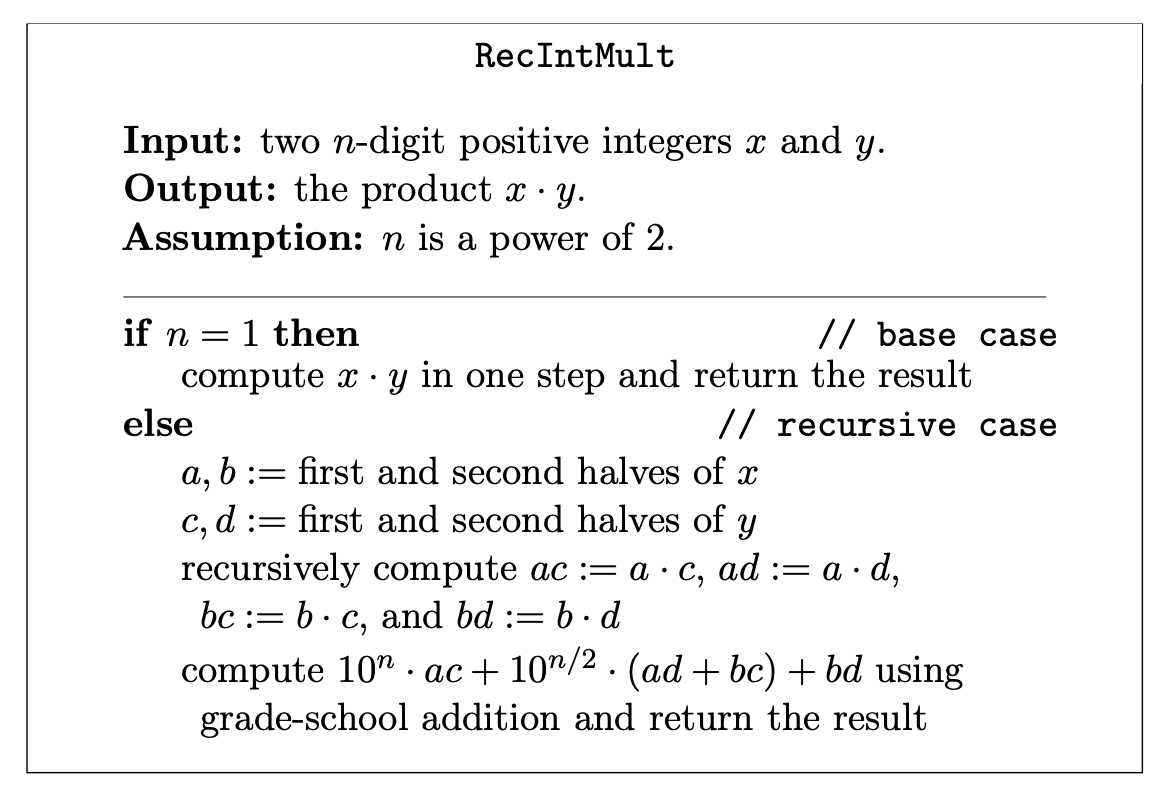
\includegraphics[scale=0.5]{recintmult.png} 
\\
\end{center}
$$T(n) \leq \underbrace{4 \cdot T\left(\frac{n}{2}\right)}_{\text {work done by recursive calls }}+\underbrace{O(n)}_{\text {work done outside recursive calls }}$$
\subsection*{The Master Theorem}
For recurrences of the form $T(n) \leq a \cdot T\left(\frac{n}{b}\right)+O\left(n^{d}\right)$,
\[
    T(n) =
    \begin{cases}
    O(n^d \log(n)) & \text{if } a = b^d\\
    O(n^d) & \text{if } a < b^d\\
    O(n^{\log_b(a)}) & \text{if } a > b^d
    \end{cases}
    \]
    where $a$ is the number of recursive calls, $b$ is the input size shrinkage factor, and $d$ is the exponent in running time of the “combine step”. (Note that the big-O values here are tight; for instance, if $\Theta(n^2)$ work is required, use $d = 2$.)
\newpage
\section{Sorting and Randomization}
\subsection*{MergeSort}
MergeSort splits a list in two halves and sorts both recursively. The merge function takes in the two sorted lists and outputs a single sorted list containing all the elements of the input lists.
 \begin{mdframed}
    \begin{minted}{python}
# Arguments: unsorted_list is an unsorted list of elements
# Return: a sorted version of unsorted_list
def merge_sort(unsorted_list):
    # base case: if list is length one, return itself
    if len(unsorted_list) == 0 or len(unsorted_list) == 1:
        return unsorted_list
    # recursive steps: recursively sort both halves
    else:
        middle_index = int(len(unsorted_list) / 2)
        left = merge_sort(unsorted_list[:middle_index])
        right = merge_sort(unsorted_list[middle_index:])
        return merge(left,right)
    
# Arguments: sorted arrays A and B (length n/2 each)
# Return: sorted array C (length n)
def merge(a, b):
    i,j = 0,0
    c = []
    while i < len(a) and j < len(b):
        if a[i] < b[j]: #need to use <= to keep stable
            c.append(a[i])
            i += 1
        else:
            c.append(b[j])
            j += 1
    # copy remaining elements into c
    c = c + a[i:] + b[j:]
    return(c)
    \end{minted}
\end{mdframed}
$$
T(n) \leq \underbrace{2 \cdot T\left(\frac{n}{2}\right)}_{\text {work done by recursive calls }}+\underbrace{O(n)}_{\text {work done outside recursive calls }},
$$
Runtime: MergeSort runs in $O(n \log n)$: the algorithm makes two recursive calls, each on an input of half the size, and performs O(n) work outside its recursive calls.
\subsection*{Partition}
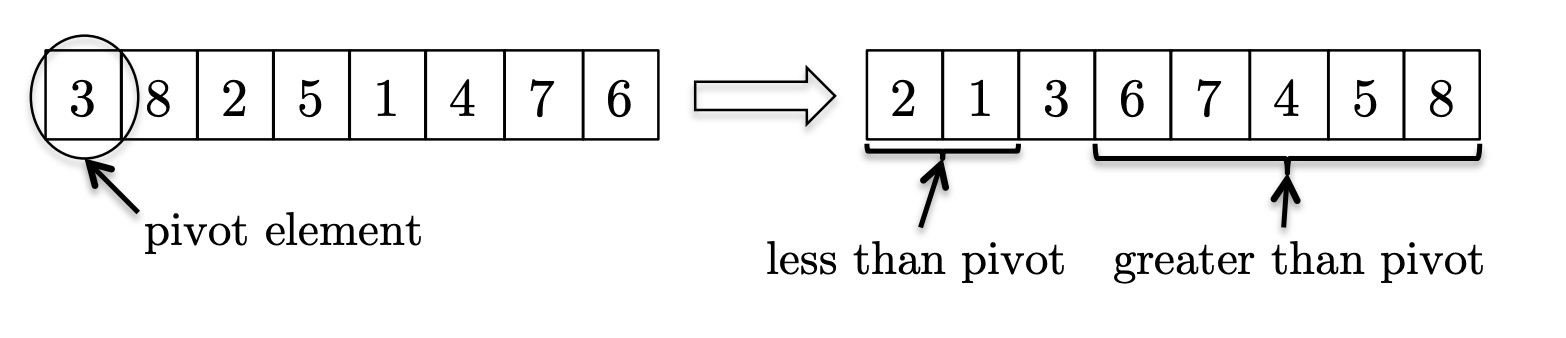
\includegraphics[scale=0.3]{partition.png}
\begin{mdframed}
\begin{minted}{python}
# divides a list into two sections around the pivot element
# returns the position of the pivot element
def partition(A, L, R, pivot):
    i = L + 1
    j = L + 1
    A[L], A[pivot] = A[pivot], A[L] # swap pivot with first element A[L]
    while j <= R:
        if A[j] < A[L]: # maintain loop invariant A[i] < pivot < A[j]
            A[i], A[j] = A[j], A[i]
            i += 1
        j += 1
    A[L], A[i - 1] = A[i - 1], A[L]  
    # swap pivot A[L] with last value less-than pivot A[i - 1]
    return i - 1 # final pivot position
\end{minted}
\end{mdframed}
Runtime: $O(n)$
\subsection*{QuickSort}
Pick an element of the list uniformly at random. Use that element as a pivot.Then recursively sort the left and right halves in the same way. \\\\
In this best-case scenario, QuickSort runs in $\Theta(n \log n)$ time. The reason is that its running time is governed by the exact same recurrence that governs the running time of MergeSort. That is, if $T(n)$ denotes the running time of this implementation of QuickSort on arrays of length $n$, then
$$
T(n)=\underbrace{2 \cdot T\left(\frac{n}{2}\right)}_{\text {since pivot }=\text { median }}+\underbrace{\Theta(n)}_{\text {ChoosePivot \& Partition }} .
$$
In the worst-case scenario, QuickSort runs in $O(n^2)$.
\subsection*{RadixSort}
\\\\
RadixSort isn't really "$O(n)$" when the number of
digits d is itself $O(\log n)$, e.g., for $b = 2$, $d = 3$, the only possible values are \texttt{000, 001, 010, 011, 100, 101, 110, 111}. If we sort a list of distinct values,
then $3 = d = \log_2n = \log_2(2^3) = 3$. Understand the idea that a comparison-based sort method can't asymptotically beat n log n, because we have $O(n!)$ leaves into a tree of decisions (one per sorting order), and the depth
ends up having to be $\Omega(n \log n)$.
\subsection*{InsertionSort}
Take the second element in the list, and as long as there is a larger element to its left, keep moving our element left. Repeat for the third, etc. elements in the list.
Insertion sort runs in quadratic $(O(n^2))$ time
\subsection*{K-select}
\begin{center}
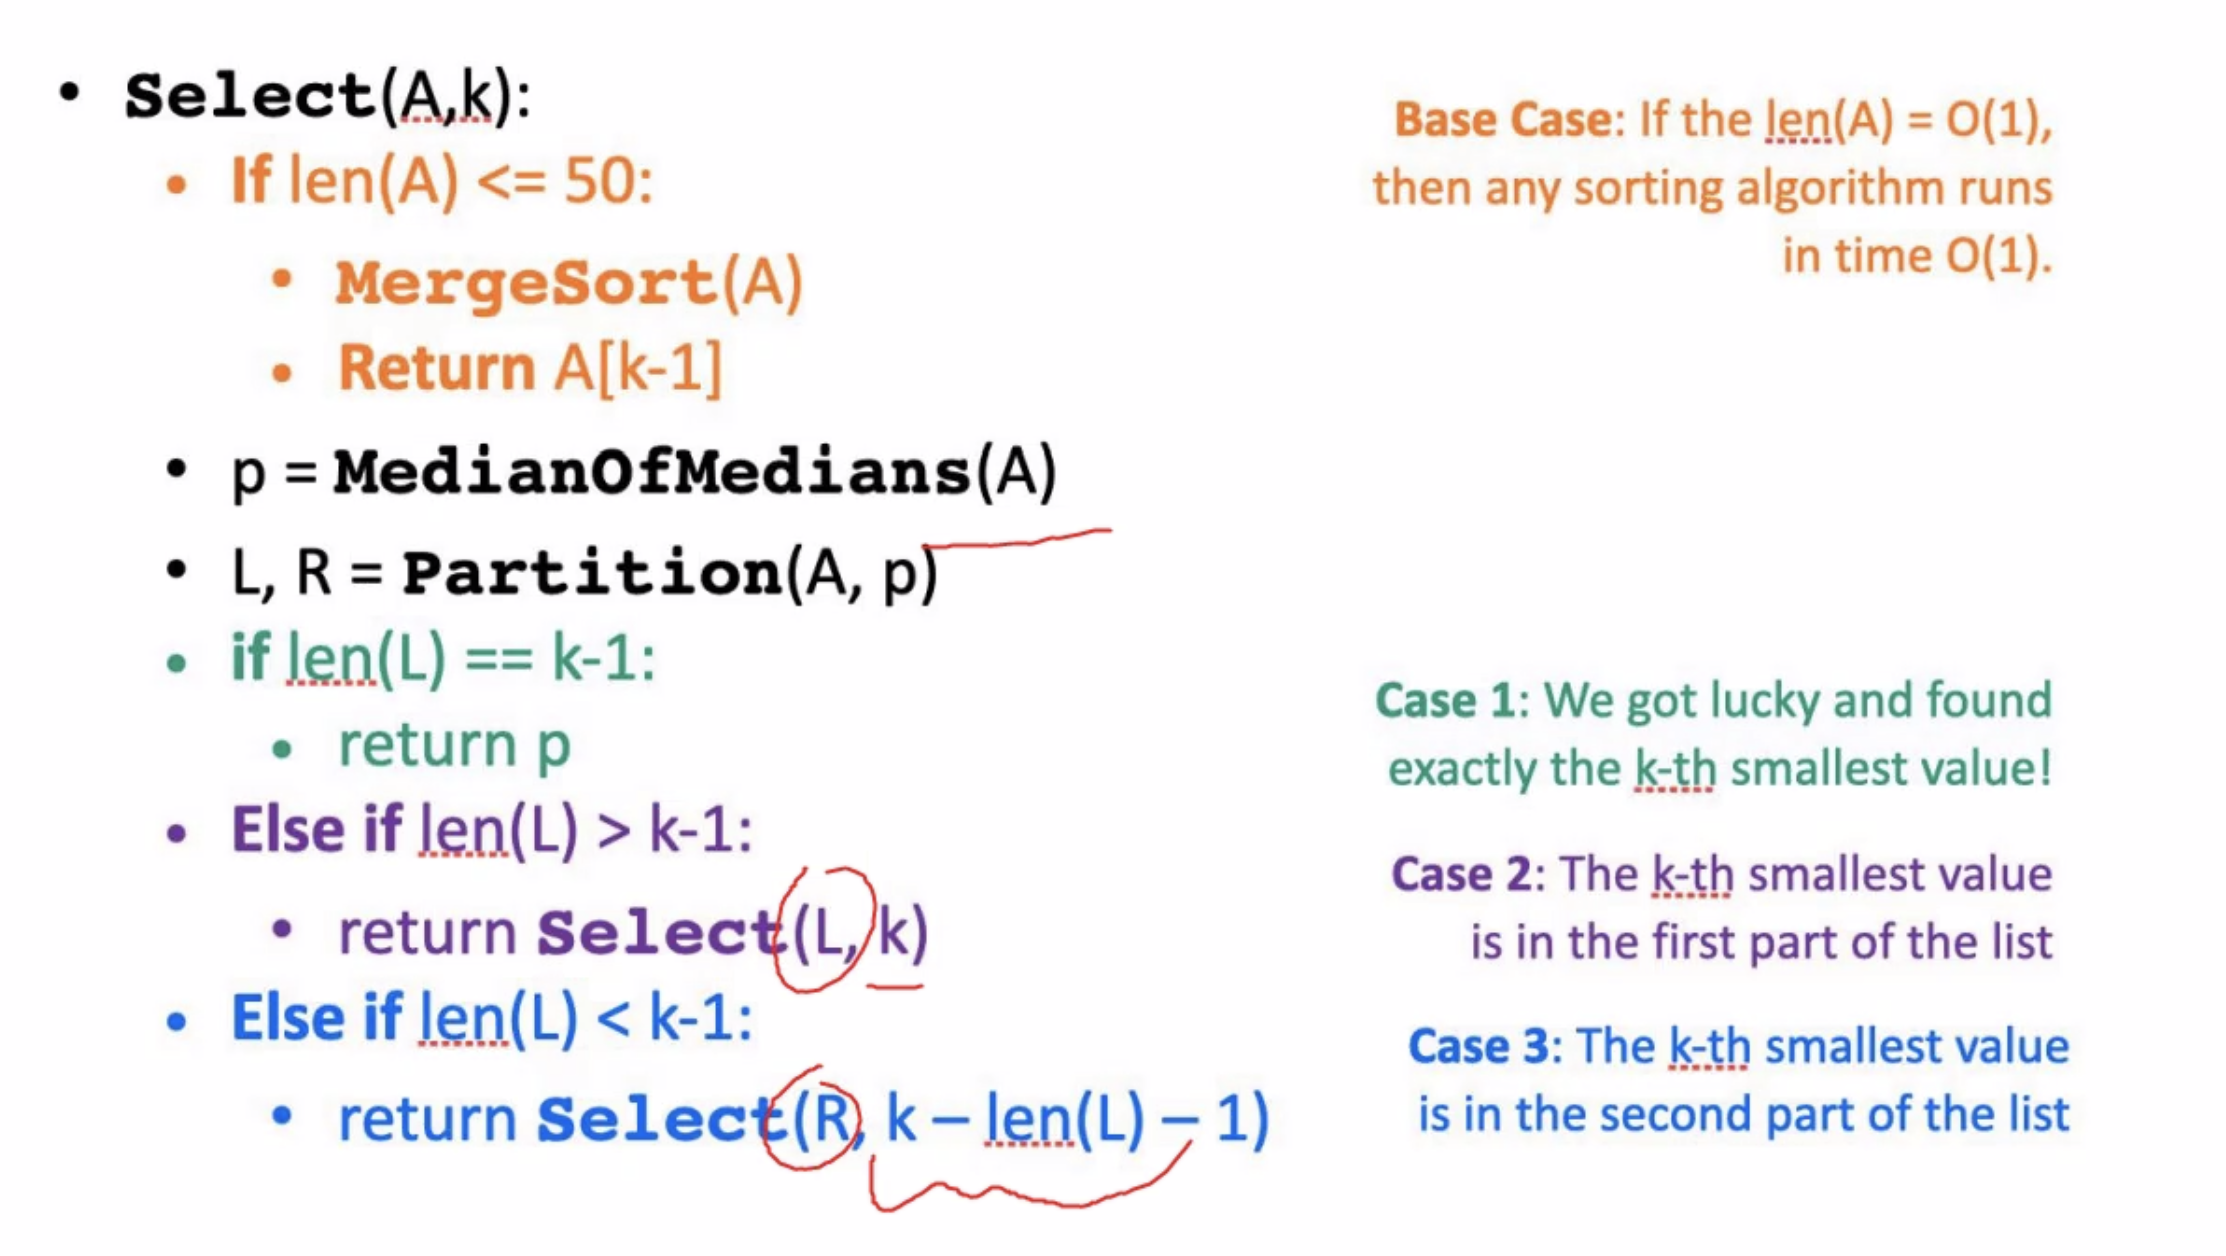
\includegraphics[scale=0.3]{select.png} \\
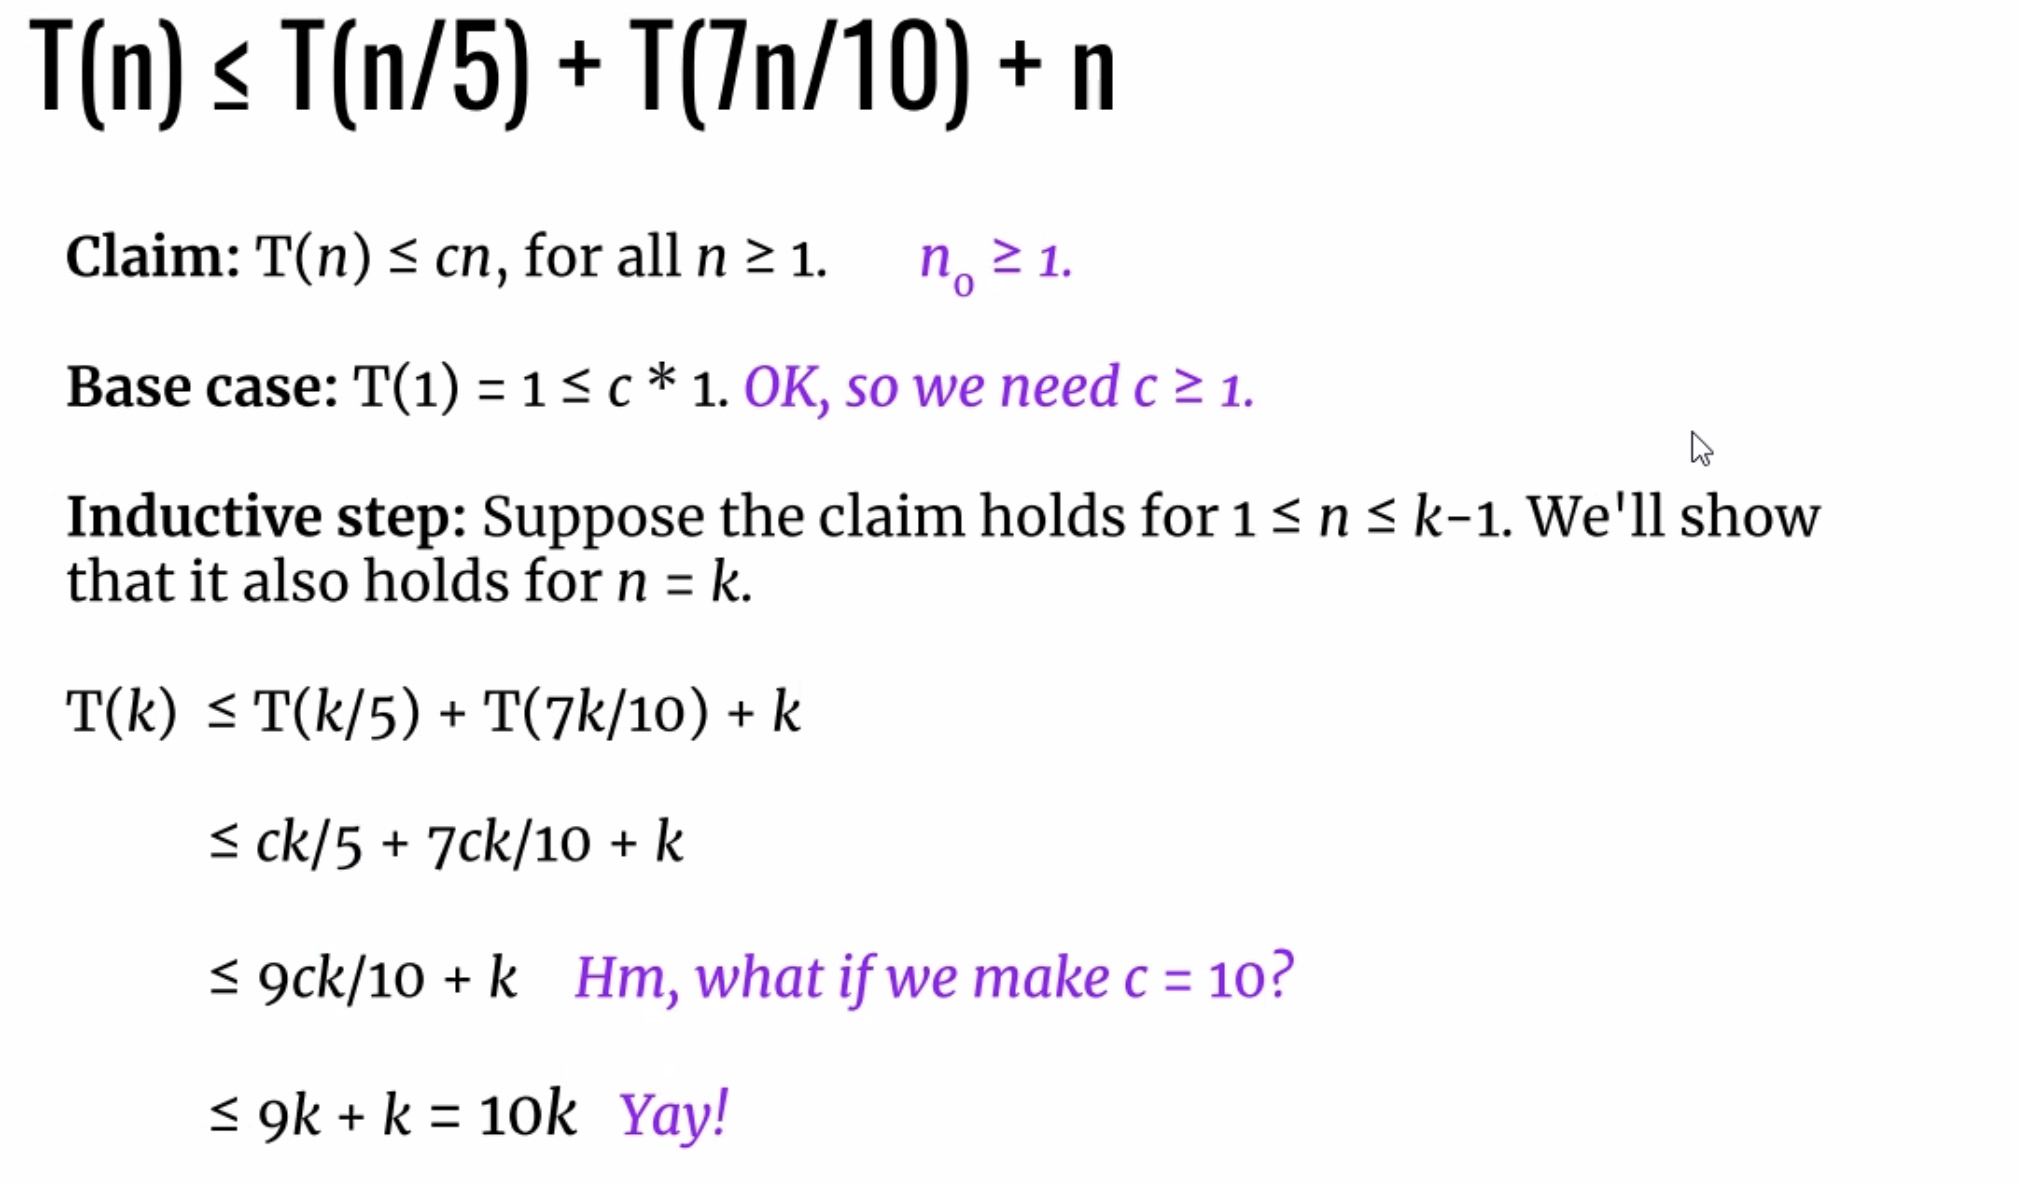
\includegraphics[scale=0.3]{kselect.png} \\
Runtime: best case is $\Omega(n)$
\end{center}
\newpage

\section{Data Structures}

\subsection*{Universal hashing}
Let $\mathcal{U}$ be the universe of all elements we could put in our hash functions, and let $\mathcal{H} = \{h_1, ..., h_m\}$ be a family of hash functions hashing these elements to $n$ buckets. Then $\mathcal{H}$ is universal if and only if for every pair $u_i, u_j$ of distinct elements in $\mathcal{U}$,
\begin{align*}
    \textbf{Pr}_{h \text{ in } \mathcal{H}} [h(u_i) = h(u_j)]  \leq \frac{1}{n}
\end{align*}
where the probability is over a (uniformly) random choice of a hash function $h$ from the family $\mathcal{H}$.
\\\\
For $i=1,2,3$, let $h_{i}(x)$ be the $i$-th least significant digit of $x$. (For example, $h_{3}(456)=4$.) Define $\mathcal{H}=\left\{h_{1}, h_{2}, h_{3}\right\}$.
\begin{tcolorbox}
Consider $x=111$ and $y=112$. Choosing $h \in H$ at random, the probability that $h(x)=h(y)$ is $2 / 3$ because $h_{2}(x)=h_{2}(y)$ and $h_{3}(x)=h_{3}(y)$.  
\end{tcolorbox}

Let $h_{a, b}(x)$ be the least significant digit of $((a x+b)$ mod 997$)$. (For example, $h_{2,3}(500)$ is the least-significant digit of $(2 \cdot 600+3) \bmod 997=206$, which is $\left.6 .\right)$ Define $\mathcal{H}=\left\{h_{i}: a \operatorname{in}\{1, \ldots, 996\}, b\right.$ in $\left.\{0, \ldots, 996\}\right\}$. (Note: 997 is prime.)

(Hint: It may help to consider $\left.\left(h_{a, b}(x)-h_{a, b}(y)\right) \bmod 997 .\right)$
\begin{tcolorbox}
This is very close to the universal hash family construction demonstrated in class, but with one crucial mistake: the prime is supposed to be larger than the size of the universe $\mathcal{U}$, not just larger than the number of buckets. As a counterexample, consider $x=000, y=997$. Then $a x+b$ is $b$ in the first case and $997 a+b$ in the second case. The difference between these two, modulo 997 , is $((997 a+b)-b \bmod 997)=(997 a \bmod 997)=0$. Therefore, these two values collide with probability 1 , regardless of the choices of $a$ and $b$.
\end{tcolorbox}
\subsection*{Bloom Filter}
What you need:
\begin{itemize}
    \item Some number $b$ of bits, all initialized to $0$.
    Some set k of hash functions $h_1, …, h_k$ that each hash to the range $[0, b-1]$.
    \item For simplicity here, we assume that when given the same element x, the hash functions all choose different values in that range $[0, b-1]$. 
\end{itemize}
Insert: add a new key k to the bloom filter. $O(1)$
\begin{itemize}
    \item Put it in every hash function" i.e., calculate $h_1
(x), …, h_k(x)$
    \item Set each bit $h_1(x), …, h_k(x) to 1$. If any of these are already 1, that's fine. They stay 1.
\end{itemize}
Lookup: for a key k, return “yes” if k has been previously
inserted into the bloom filter and “no” otherwise. $O(1)$
\begin{itemize}
    \item Put it in every hash function - calculate $h_1(x), …, h_k(x)$
    \item Check each bit $h_1(x), …, h_k(x)$
    \item If at least one of these is 0, we have definitely not seen this item before
\end{itemize}
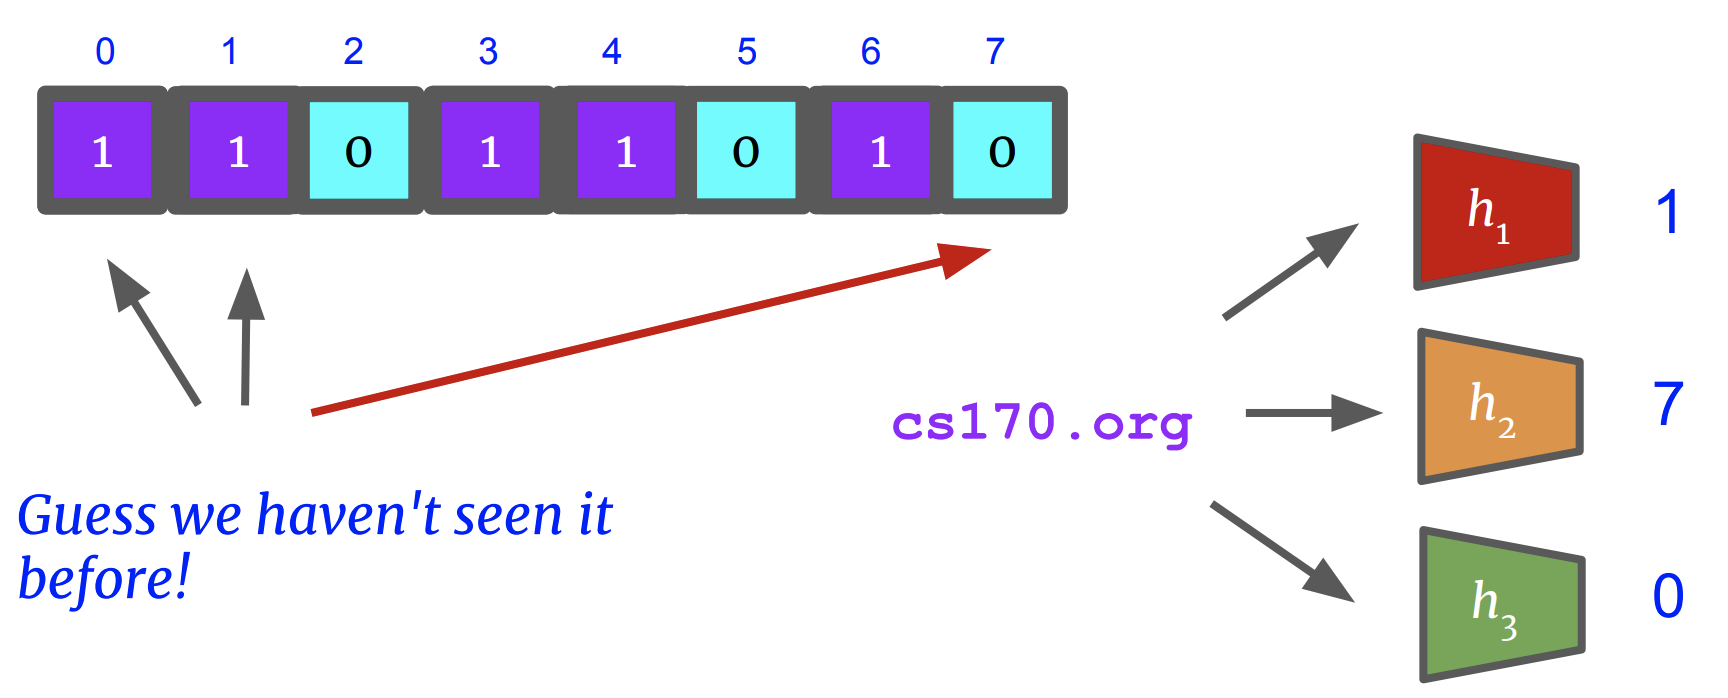
\includegraphics[scale=0.5]{bloomfilter.png} 
\subsection*{Binary search trees}
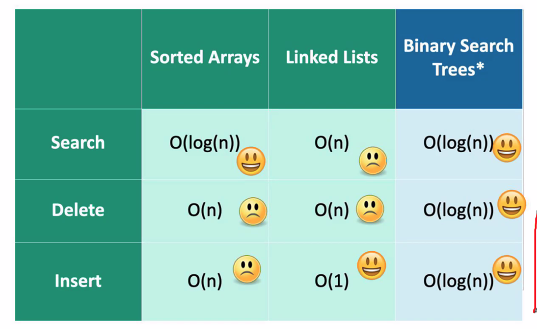
\includegraphics[scale=0.5]{bst.png} 
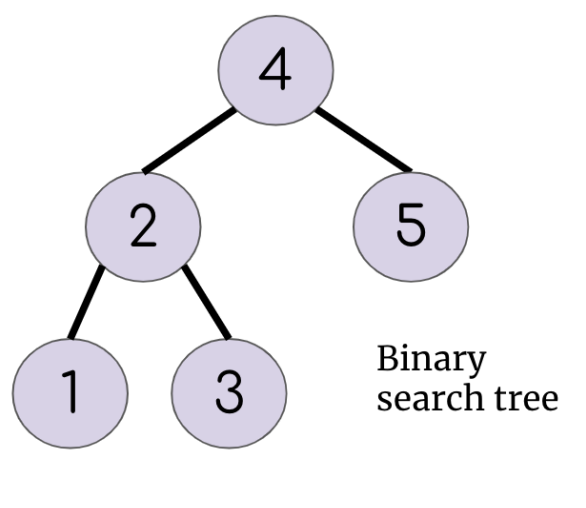
\includegraphics[scale=0.5]{smallbst.png} 
\\ These are labeled binary trees such that:
\begin{itemize}
    \item the values of any node's left child (and all its descendants) are all no greater than the node's own value
    \item the values of any node's right child (and all its descendants) are all no smaller than the node's own value
\end{itemize}
What's special: supports search, delete, insert
\subsection*{Binary heaps}
Every node's value is no larger than the values of all its children.
\begin{center}
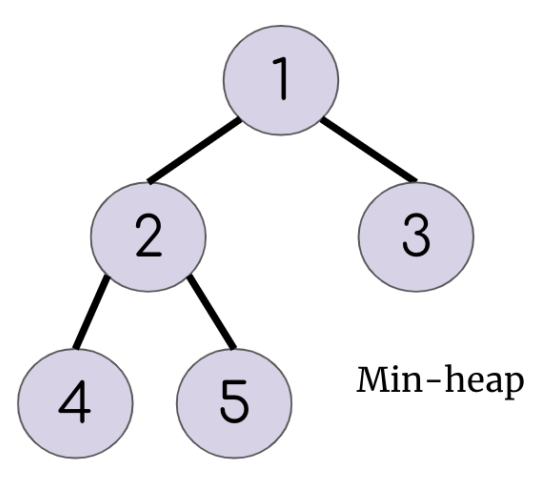
\includegraphics[scale=0.5]{minheap.png} 
\end{center}
What's special: 
\begin{itemize}
    \item You can peek at the min in constant time
    \item Insertion and deletion are $O(\log(n))$ because we're bubbling up / bubbling down. 
    \item Search is not supported :( 
\end{itemize}
\subsection*{Red-black tree rules}
\begin{itemize}
    \item Every node is colored red or black.
    \item The root node is a black node.
    \item Any missing children (a leaf has two of these, an internal node with only one child has one of these) are NILs that count as black nodes.
    \item Children of a red node are black nodes.
    \item For any node $x$, all paths from $x$ to NILs have the same number of black nodes.
\begin{center}
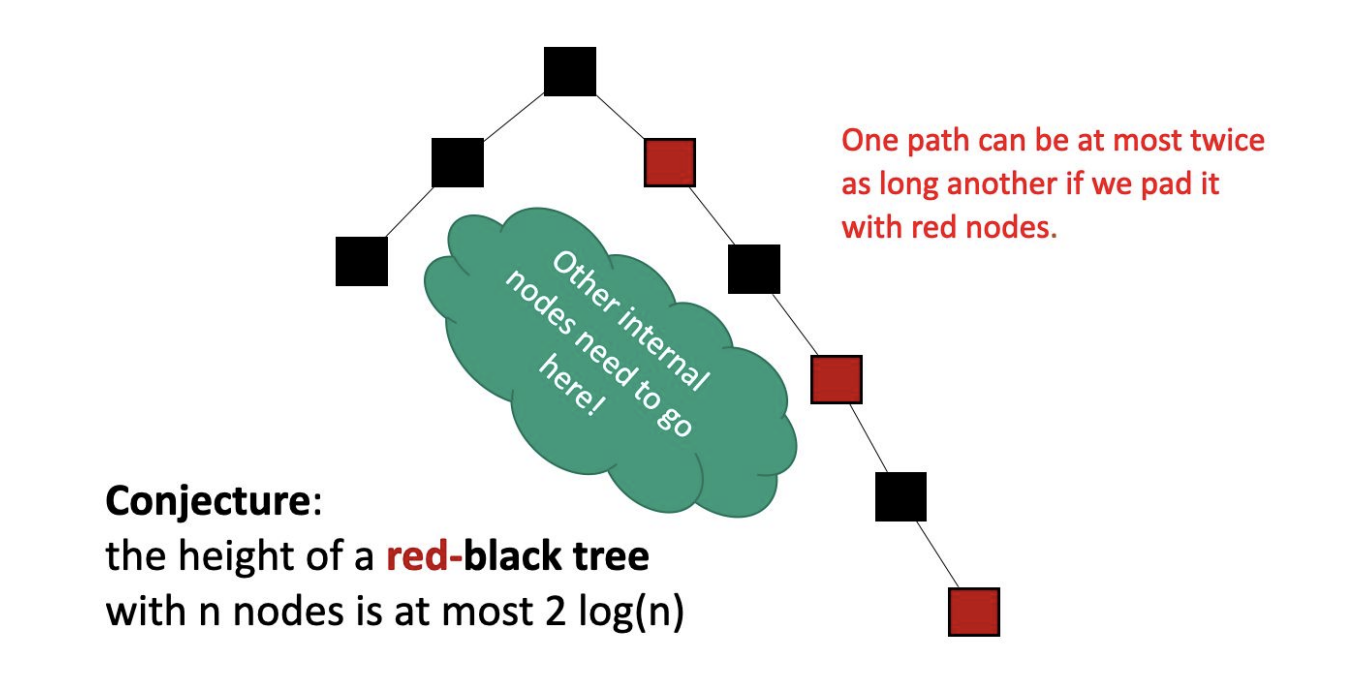
\includegraphics[scale=0.5]{rbtbalance.png} 
\end{center}
\end{itemize}
What's special: search, insertion, deletion are all $O(\log(n))$ because of the depth guarantee. 
\subsection*{Fibonacci heap}
\begin{center}
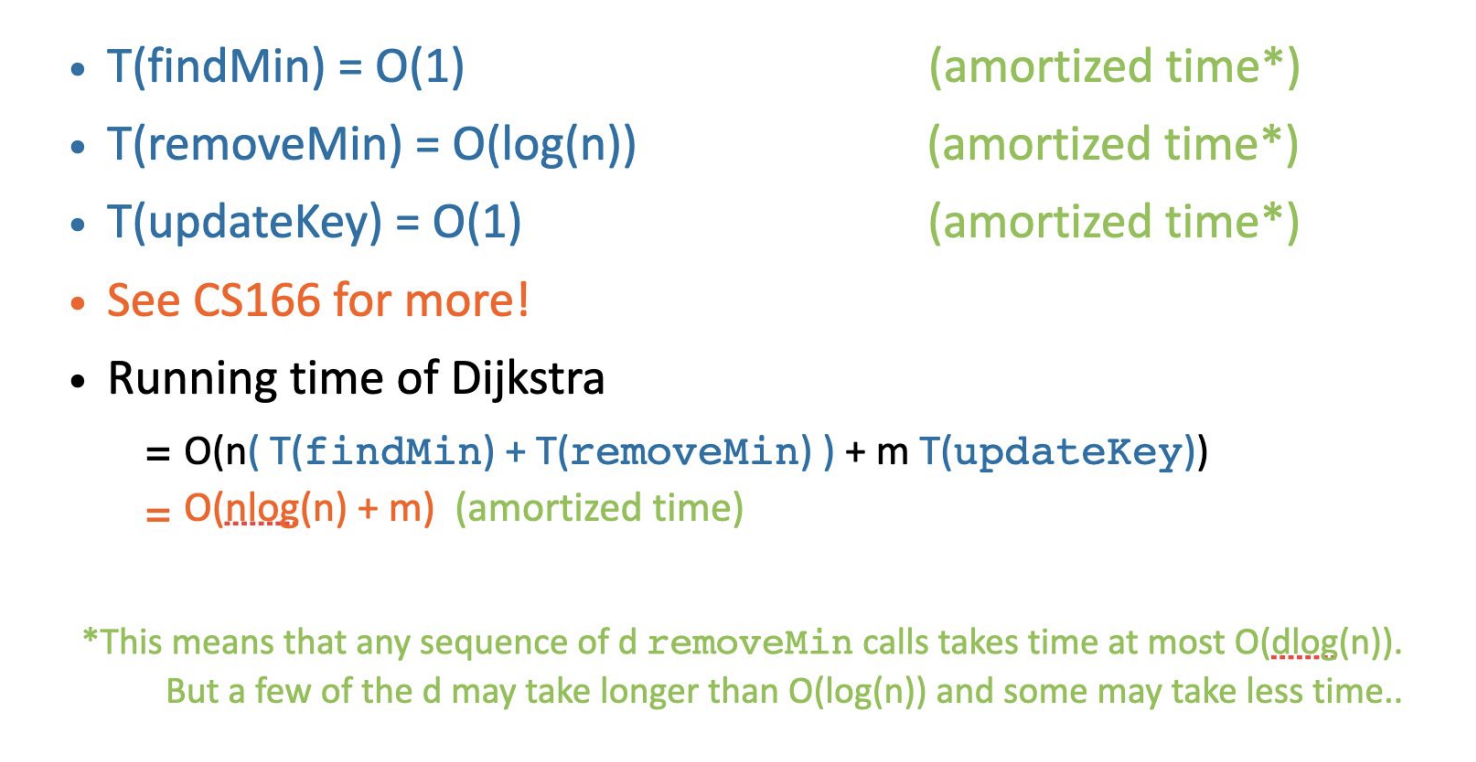
\includegraphics[scale=0.5]{fibonacci.png} 
\end{center}
\subsection*{Binary search}
Pseuodocode: First check if the object in the middle position of the array has the desired key. If so, return it. If not, recurse either on the left half (if the middle object’s key is too large) or on the right half (if it’s too small).
\begin{mdframed}
\begin{minted}{python}
def binarySearch(arr, l, r, x):
    # Check base case
    if r >= l:
        mid = l + (r - l) // 2
        # If element is present at the middle itself
        if arr[mid] == x:
            return mid
        # If element is smaller than mid, then check left
        elif arr[mid] > x:
            return binarySearch(arr, l, mid-1, x)
        # Else check right
        else:
            return binarySearch(arr, mid + 1, r, x)
    else:
        # Element is not present in the array
        return -1
\end{minted}
\end{mdframed}
Runtime: $O(\log n)$.
\begin{mdframed}
\begin{minted}{python}
def binarysearch(alligatorlist, n, W):
    current_alligator = int((len(alligatorlist))/ 2)
    # check current alligator
    if checkAlligator(n, W, alligatorlist[current_alligator]):
        # check again with the next largest alligator
        if current_alligator+1 < len(alligatorlist) and checkAlligator(n, W, alligatorlist[current_alligator + 1]):
            # if true, alligator is too small
            return binarysearch(alligatorlist[current_alligator+1:], n, W)
        else:
            # if false, we have found the optimal alligator! return cur
            return alligatorlist[current_alligator]
    else: #try a smaller alligator
        return binarysearch(alligatorlist[:current_alligator], n, W)
\end{minted}
\end{mdframed}
\newpage
\section{Graph Search}
\subsection*{Graphs}
\begin{itemize}
    \item $n$ \textbf{nodes}, $m$ \textbf{edges}
        \begin{itemize}
        \item There are $\binom{n}{2} = \frac{n(n-1)}{2}$ pairs of vertices, so there can be up to that many edges as well!
        \item edges can be \textbf{directed} or \textbf{undirected}
        \\ 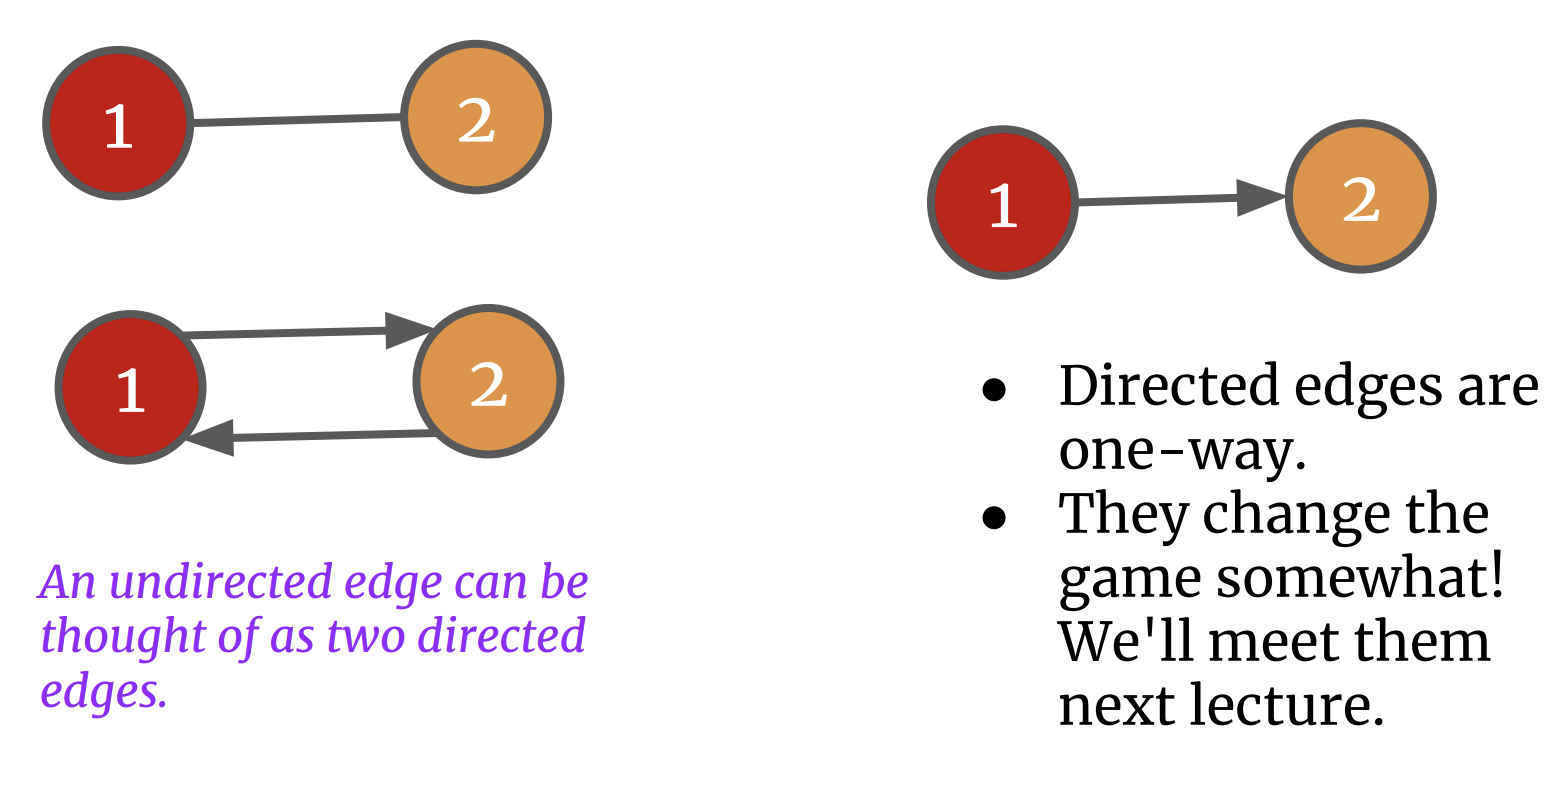
\includegraphics[scale=0.2]{directed.png}
        \end{itemize}
    \item \textbf{connected component}
        \begin{itemize}
            \item This graph has three connected components \\ 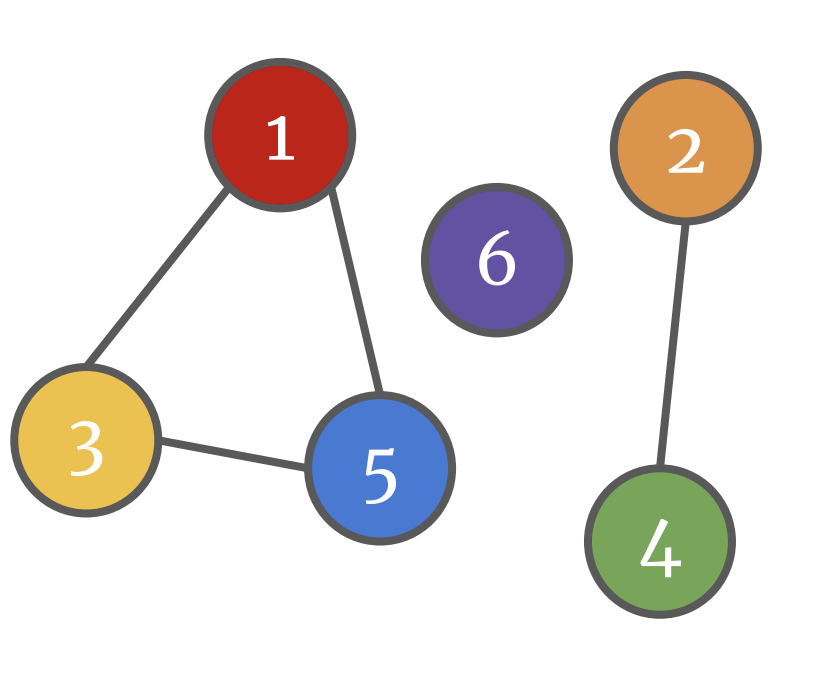
\includegraphics[scale=0.2]{connectedcomponent1.png}
            \item \textbf{connected graphs} have one connected component and (at least one) path between any two vertices. \\\\ 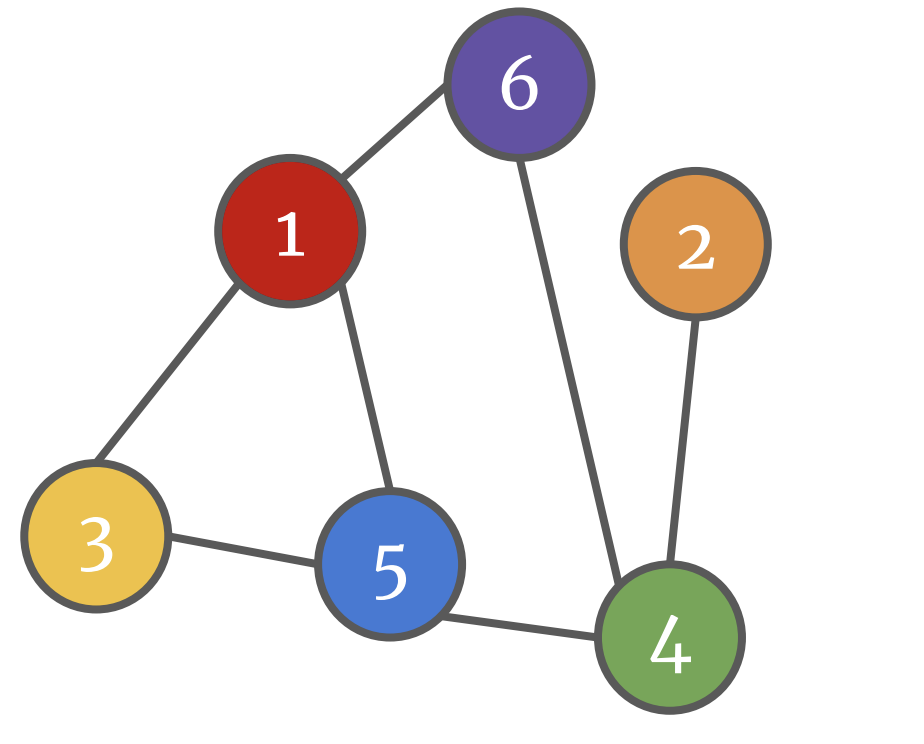
\includegraphics[scale=0.2]{connected.png}
            \item we can count connected components with the following algorithm: Proceed through the vertices in order 1, 2, …, doing the following: if a vertex has not been SEEN, perform a breadth-first traversal on it and mark all encountered nodes as SEEN; increment the count of connected. Otherwise, do nothing.
            \item a \textbf{strongly connected component} (SCC) is a maximal set of nodes in a directed graph; each node is reachable from all of the others in the SCC. 
            \begin{itemize}
                \item SCCs break a graph down into little self-contained universes. This matters a lot in, e.g., social networks.
            \end{itemize}
            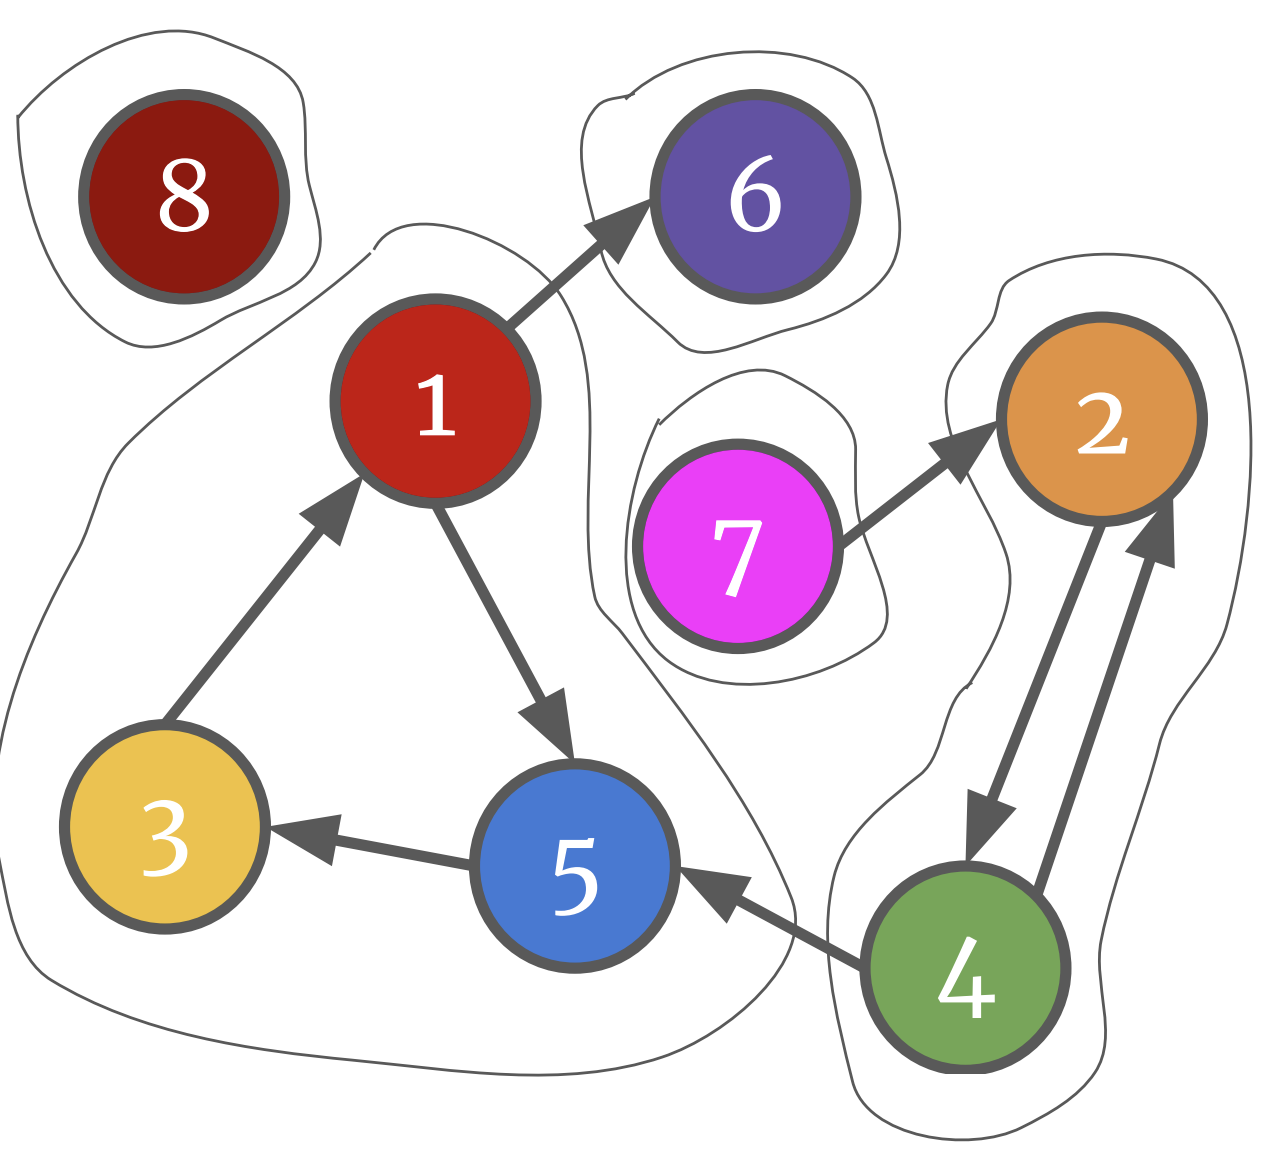
\includegraphics[scale=0.2]{scc.png}
            \end{itemize} 
    \item \textbf{bipartite graphs}
        \begin{itemize}
            \item a graph is \textbf{bipartite} if it can be divided into exactly two groups, such that every edge goes between the groups (i.e., no edges within groups)
            \item bipartiteness is the basis of matching problems. e.g., suppose that the vertices on the top are people, and the vertices on the bottom are jobs, and edges show who can do what. Can we give everyone exactly one job?
            \\ 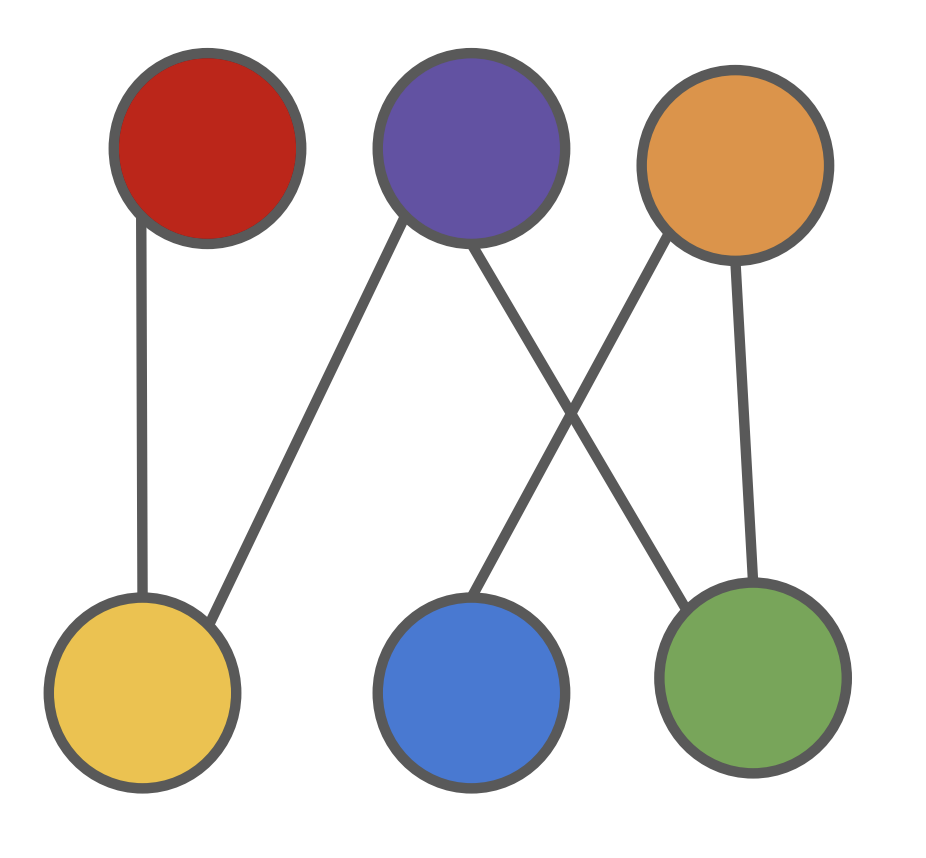
\includegraphics[scale=0.2]{bipartite.png}
            \item This is also the basis of problems like: You know of a bunch of pairs of people who won't work together. Can you split them into two groups while honoring all of their requests?
            \\ 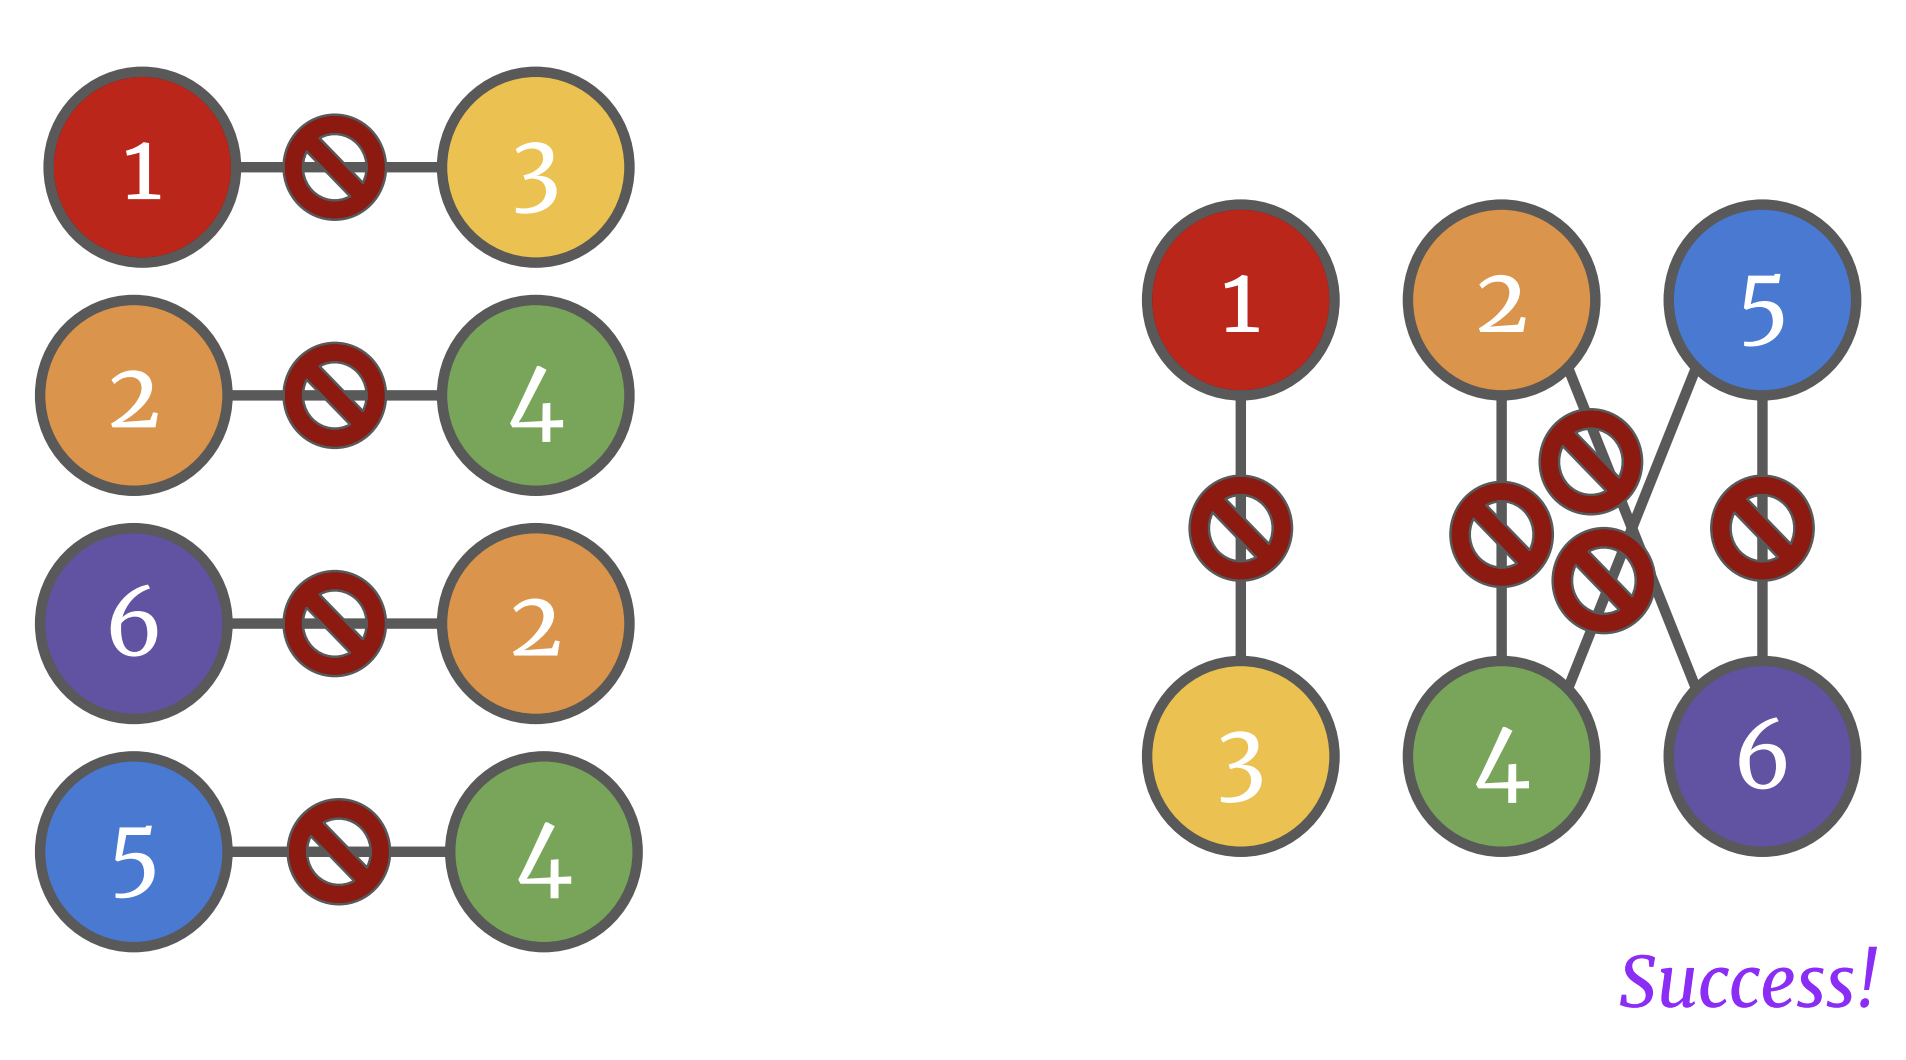
\includegraphics[scale=0.2]{bipartite2.png}
            \item a graph is bipartite if and only if it has no odd cycles.
            \\ 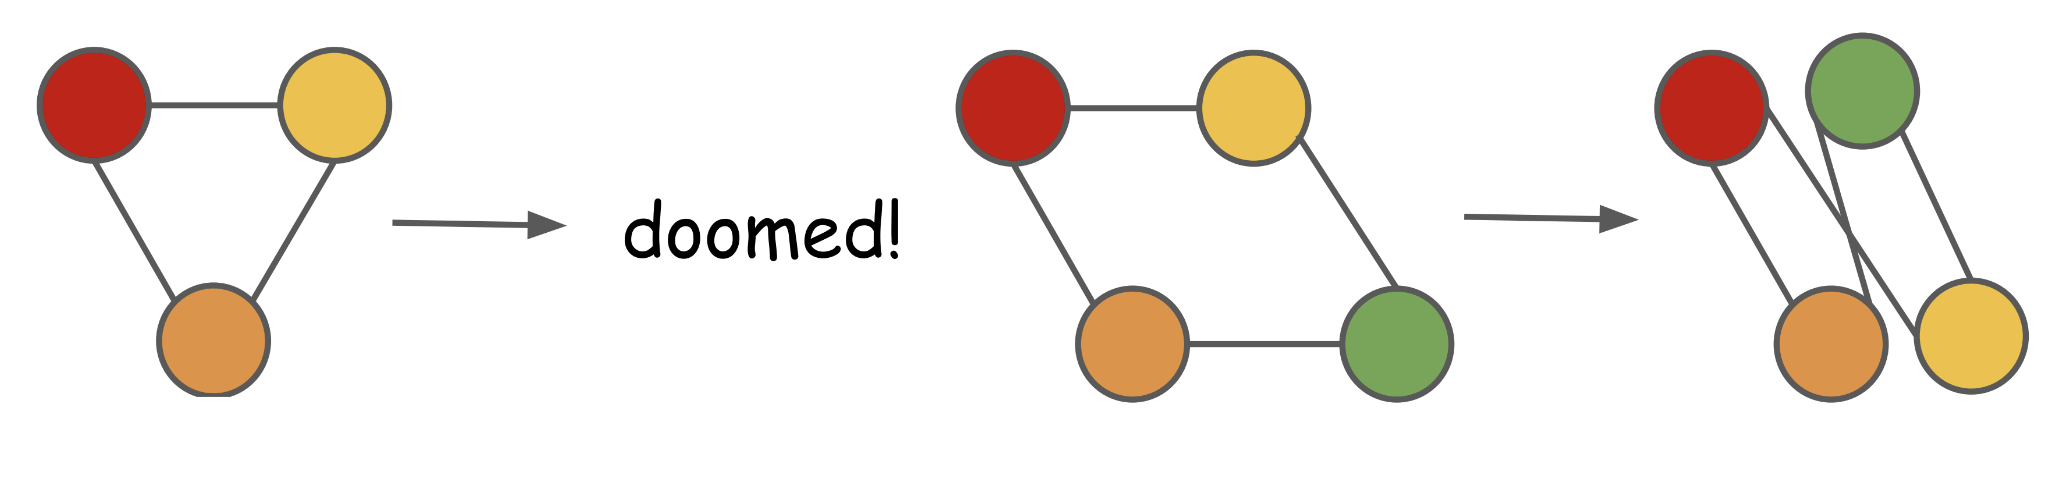
\includegraphics[scale=0.3]{bipartiteoddcycles.png}
        \end{itemize}
    \item \textbf{directed graphs}
    \begin{itemize}
        \item Node 7 is a \textbf{source} since it has no incoming edges. 
        \item Node 6 is a \textbf{sink} since it has no outgoing edges. 
        \\ 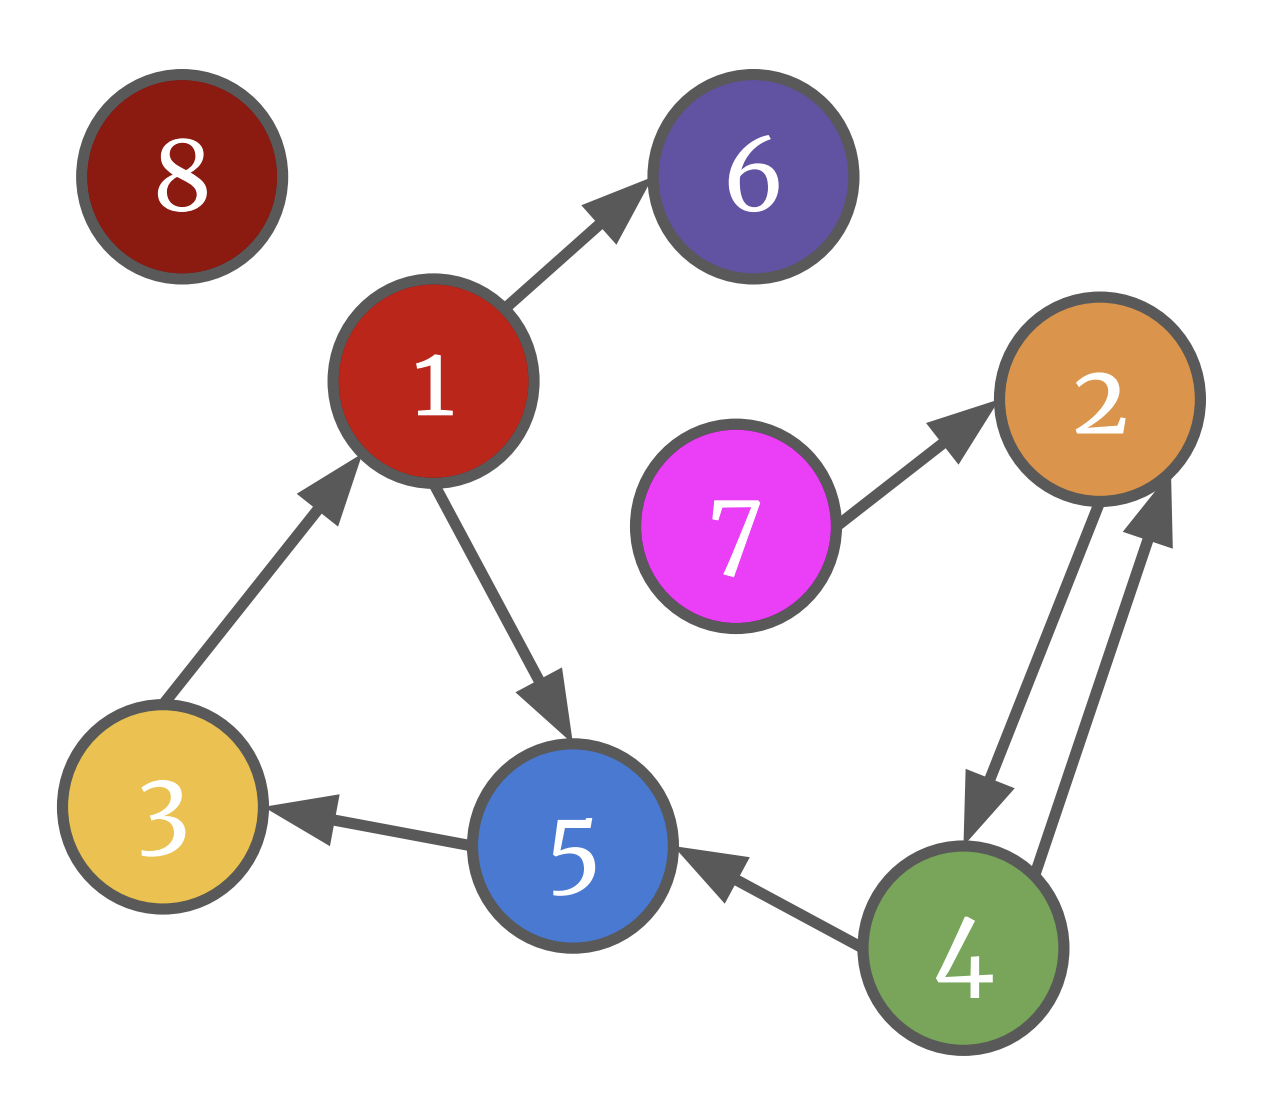
\includegraphics[scale=0.2]{sourcesink.png}
    \end{itemize}
\end{itemize}
\subsection*{Breadth-first Search (BFS)}
Goal: Traverse every node. Or, what can you reach? \\\\
TL;DR: Visit all vertices that are directly connected to the start vertex. Then visit all vertices that are directly
connected to those vertices. \\\\
Pseudocode
\begin{itemize}
    \item Create a \textbf{queue} of vertices to visit. Initially, Add the starting vertex and mark as INSERTED.
    \item Repeat the following:
    \begin{itemize}
        \item Pop off the first value in the queue.
        \item Follow each of its edges (in some order), putting the vertices you find in the queue (and marking them as INSERTED) as long as they are not INSERTED
    \end{itemize}
\end{itemize}
Runtime: You consider each edge ($m$) and each vertex ($n$) at least once, so it takes $O(m + n)$. \\\\
Notes:
\begin{itemize}
    \item Good for "shortest distance" type questions
\end{itemize}

\subsection*{Depth-first search (DFS)}
TL;DR: Stack-based. Kinda like in BFS, keep track of which nodes have been visited. Keep visiting an unvisited
neighbor (breaking ties by, e.g., node number). Backtrack whenever we are out of options. \\\\
Runtime: Like in BFS, we considered each edge at most twice –
once on the way "out", and once on the way
"back". Also like in BFS, we had to look at all the neighbors of each node. (Once we have done this once, we can advance through the list instead of looking again) So: $O(n + m)$, like BFS. \\\\
Notes
\begin{itemize}
    \item Good for in-order traversal for trees, especially binary search tree
    \item Some algorithms, like topological sort rely on DFS and its stack-based operation.
    \item DFS is also one way to solve a classic problem called 2-SAT
\end{itemize}

\subsection*{Dijkstra's Algorithm}
Goal: Find the lowest-cost path from A to B. 
\begin{itemize}
    \item Network routing: how should we send packets? (OSPF, a routing protocol for IP networks, uses Dijkstra)
    \item What is the shortest path from Palo Alto to [anywhere else]? Edge weights are time, money, hassle.
\end{itemize}
Pseudocode:
\begin{center}
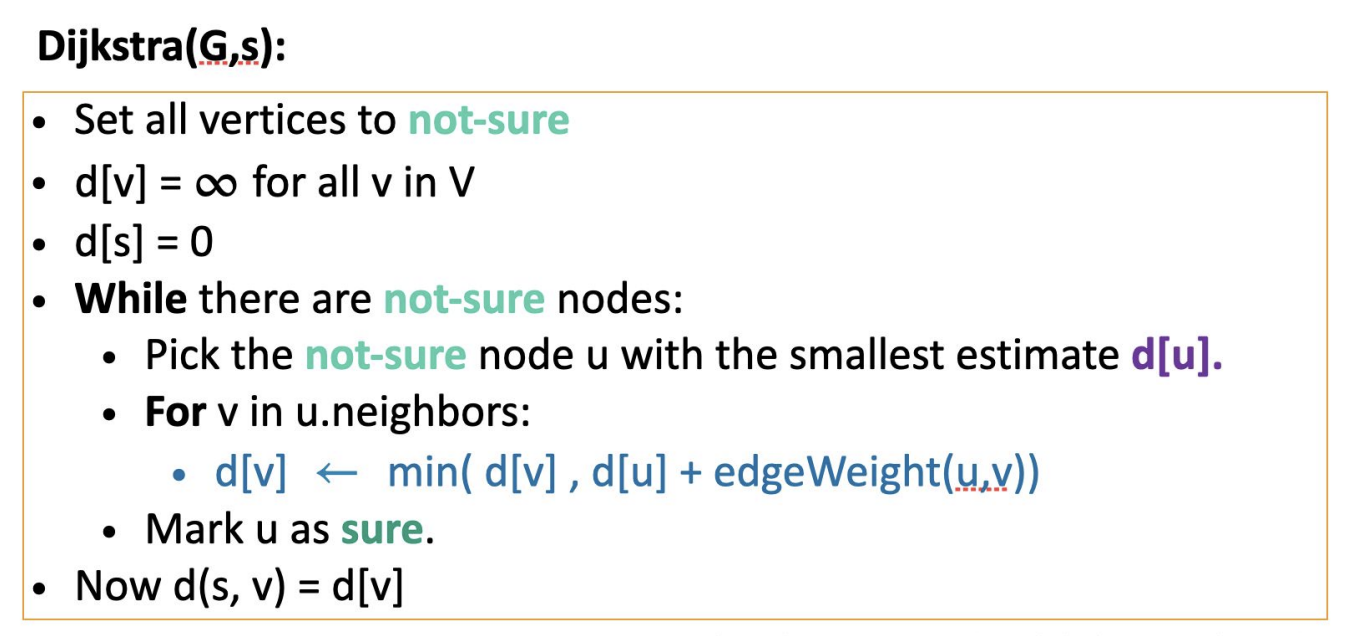
\includegraphics[scale=0.5]{dijkstra.png} 
\\
This process is called relaxing an edge.
\end{center}
Runtime: Dijkstra’s normally runs in $O(n \log n + m)$ time. The log factor comes from the use of a heap
\\\\
Notes:
\begin{itemize}
\item Cannot handle negative weights: marks a node as sure when it has considered all the paths that could be better, under the assumption that there are no negative weight edges, not all the paths overall; when there are negative weight edges, there are paths that could be better because of various assumptions (score will never decrease)
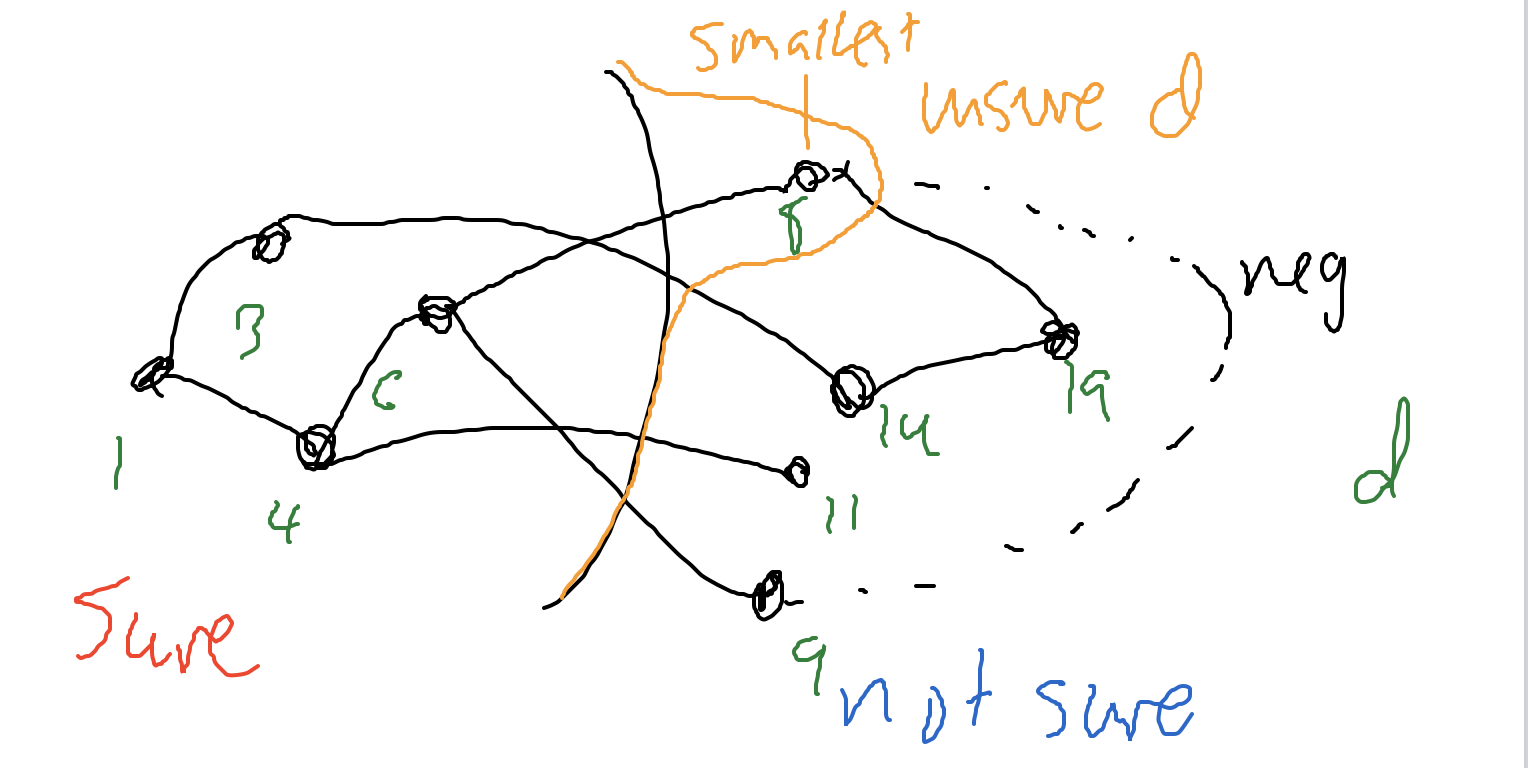
\includegraphics[scale=0.3]{dijkstranegative.png} 
\\
\item Need to rerun if weights change ("front" would advance differently - have to update everything)
\end{itemize}

\subsection*{Topological sort}
Goal: Find a valid ordering of a directed acylic graph (e.g. an order for taking classes). 
\\\\
Pseudocode: First, do a DFS, but keep track of when we start
and finish each node. Then take the finishing times in reverse order.
\\\\
Runtime: Same running time as DFS: $O(n + m)$. We don't need to sort the list of finishing times at the end. We can just record nodes as they finish.
\\\\
Notes:
\begin{itemize}
    \item Why does this work? If node A finishes before node B, there cannot be a path from A to B. (We don't say a node is done until we've fully explored all its descendants.)
    \item Sensitive to start location and tiebreak rules, but can never give a wrong answer 
\end{itemize}

\subsection*{Kosaraju's Algorithm}
Goal: Find strongly connected components in a directed graph.
\\\\
Pseudocode: 
\begin{center}
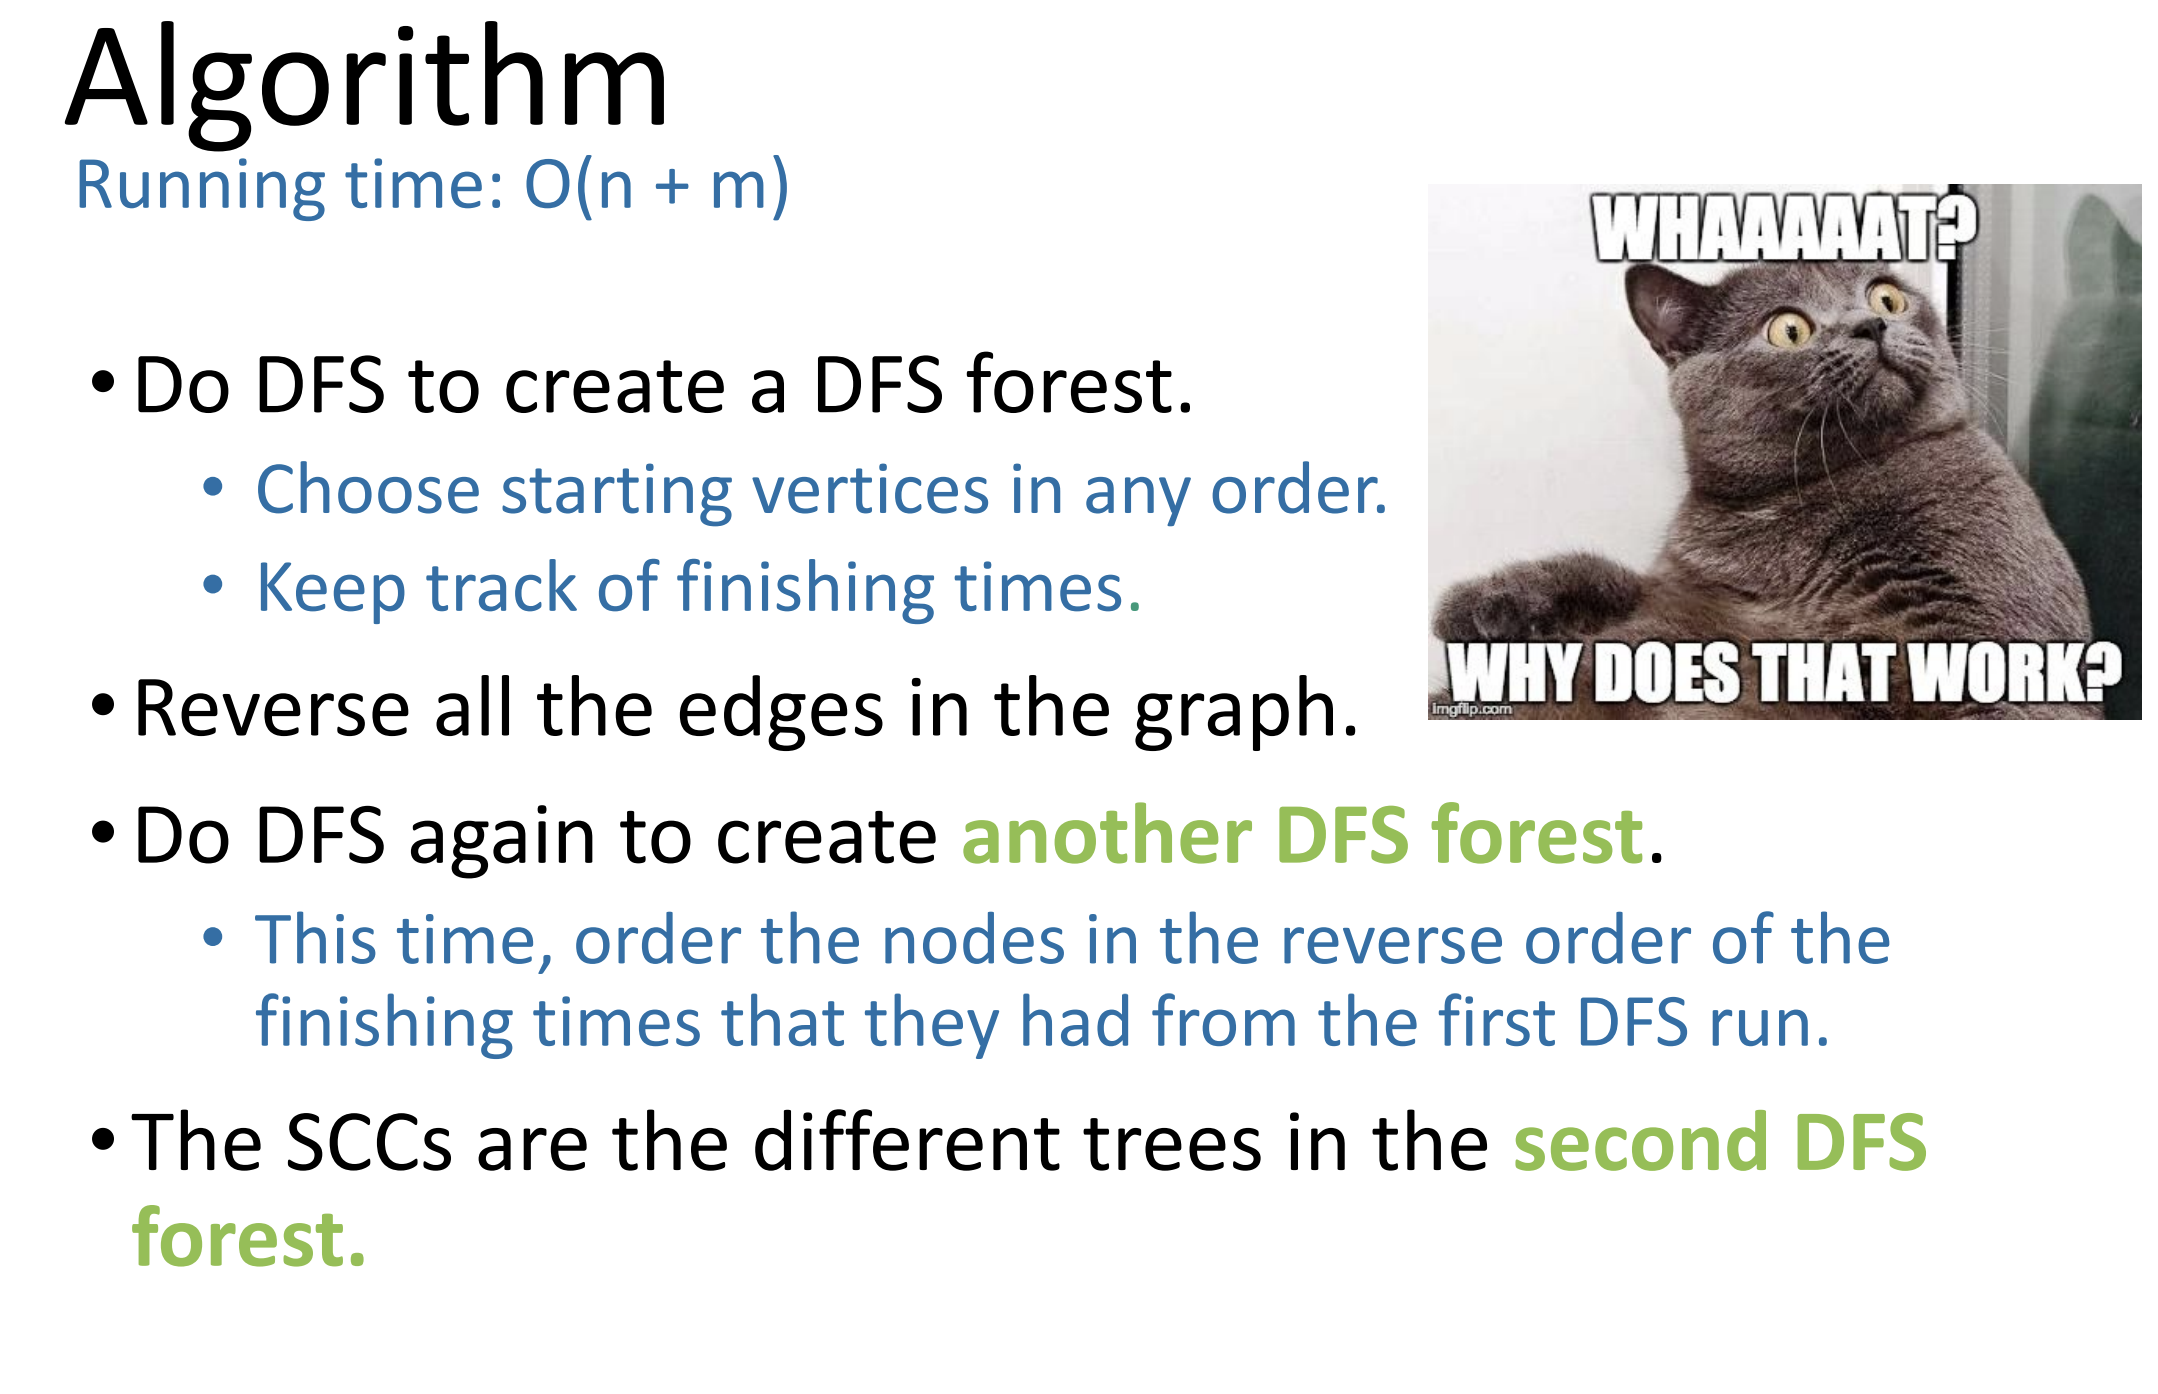
\includegraphics[scale=0.3]{kosaraju.png} 
\end{center}
Runtime: $O(n + m)$.
\\\\
Notes:
\begin{itemize}
    \item if there was a cycle among the SCC graphs, then becuase you can get from one cluster to another cluster, it would just be one massive SCC; therefore, if you collapse the SCCs into vertices, the resulting graph should not have any cycles 
    
\end{itemize}

\subsection*{Karger's Algorithm}
Goal: Randomized approach to min cut. 
\\\\
Pseuodocode: Repeat the following until there are only two vertices left in the graph:
\begin{itemize}
    \item Select an edge uniformly at random from all remaining edges. (not from all remaining pairs of vertices) Contract that edge.
    \item Return the set of edges between the vertices as the min cut.
\end{itemize}
\begin{center}
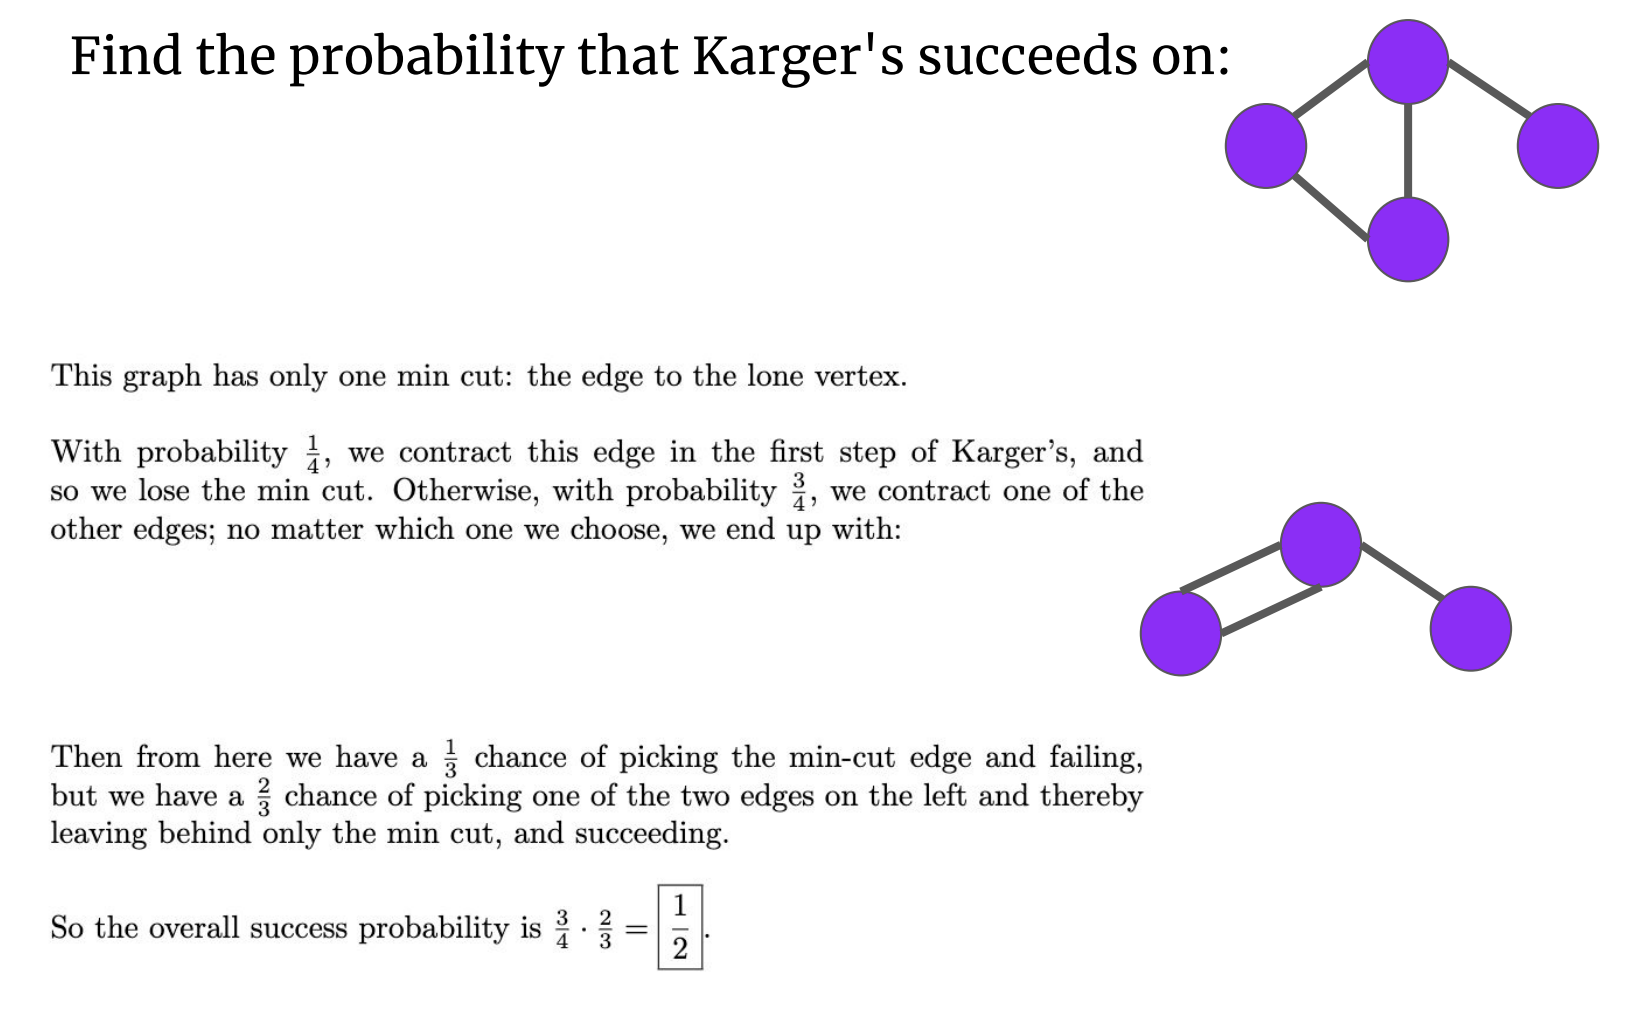
\includegraphics[scale=0.3]{kargerex.png} 
\end{center}

\newpage
\section{Dynamic Programming}
Find some substructure and exploit it to do avoid doing redundant work. 

\begin{mdframed}
\center{\textbf{The Dynamic Programming Paradigm}}
\begin{enumerate}
    \item Identify a relatively small collection of subproblems. 
    \item Show how to quickly and correctly solve "larger" subproblems given the solutions to "smaller" ones. 
    \item Show how to quickly and correctly infer the final solution from the solutions to all of the subproblems. 
\end{enumerate}
\end{mdframed}

\begin{itemize}
    \item \textbf{Top-down}: Start from the original problem (what you want), e.g., Fib(5). Remember the solutions to subproblems (memoization). - ex. edit distance
    \item \textbf{Bottom-up}: Start from the base case(s), e.g., Fib(0) and Fib(1). Use these to compute Fib(2), then use this info to compute Fib(3), etc. ex. knapsack
    \item Bottom-up is often a better choice since it avoids the overhead of lookups and storing a bunch of intermediate data. But it's also often harder to write.
\end{itemize}

\subsection*{Bellman-Ford}
Goal: Find shortest path from a source (only one starting point) to a destination for \textbf{directed} graphs. Can handle negative edge weights. 
\\\\
Pseudocode: Check all the edges in some arbitrary order and update distance. Do this at most $n-1$ times (because the longest path without cycles is $n-1$ if there are n nodes), then one extra time (to check if there is a negative cycle)
\\\\
Runtime: 
\begin{itemize}
    \item We do $n$ rounds of looking at m edges each.
    \item Each check of an edge (and update of the destination' estimate and predecessor) takes $O(1)$ time.
    \item Therefore: $O(nm)$ overall. For a dense graph with $m = O(n^2)$, could be $O(n^3)$
\end{itemize}
\\\\
Notes:
\begin{itemize}
    \item Why do negative edges matter? 1) Profits and costs for performing certain actions. 2) Elevation - electric cars use energy on uphills, regenerate on downhills. 
\end{itemize}

\subsection*{Floyd-Warshall}
Goal: Find shortest paths \textbf{between all pairs of vertices} in a weighted directed graph; holds all of this in some data structure
\\\\
tl;dr: A series of increasingly good estimates. First round - either use direct edge between two vertices, or use I as intermediate. Second round - either direct edge, or use I and II as intermediate.
\\\\
Pseudocode: The algorithm operates in $n$ rounds, and in each $k$-th round, for every ordered pair of vertices in the graph, it asks the following: What is the shortest path between these two vertices that is either a direct connection, or only visits intermediate vertices numbered $k$ or smaller? (``Intermediate" vertices specifically do not include the two ends of the path.) 
\\\\
In the first round of Floyd-Warshall, we are considering using just vertex as an intermediate vertex. For each ordered pair $(i, j)$ of vertices -- possibly with $i = j$ -- we consider whether the total cost of going from vertex $i$ to vertex I to vertex $j$ is less than the cost of going from directly from vertex $i$ to vertex $j$.
\\\\
The algorithm keeps track of an $n \times n$ matrix $A$. The $j$-th cell of the $i$-th row of $A$ -- that is, $A_{ij}$ -- represents the current best estimate of the minimum total cost to go from vertex $i$ to vertex $j$. The cells on the diagonal (the $A_{ij}$ for which $i = j$) are initialized to $0$. Every other cell $A_{ij}$ is initialized to $\infty$ if there is no edge from vertex $i$ to vertex $j$, or to the weight of that edge otherwise.
\begin{align*}
    \begin{bmatrix}
    0 & -2 & \infty & 4\\
    \infty & 0 & \infty & 1\\
    4 & 3 & 0 & \infty\\
    1 & \infty & \infty & 0\\
    \end{bmatrix}
\end{align*}
Runtime: We carry out $n$ rounds, each of which involves going through an $n \times n$ matrix and doing $O(1)$ work. Overall, this is $O(n^3)$.
\\\\
Notes:
\begin{itemize}
    \item fill this in later
\end{itemize}
\subsection*{Knapsack problem}
Goal: use a scarce resource in the smartest way problem
\\\\
Pseudocode:
\\\\
Runtime:
\\\\
Notes:
Some examples:
\begin{itemize}
    \item Which goods and services should you spend your paycheck to get the most value?
    \item Given an operating budget and a set of job candidates with differing productivity and requested salaries, whom should you hire? 
\end{itemize}
bottom up DP algorithm
\subsection*{Longest common subsequence}
\begin{mdframed}
\begin{minted}{python}
def longestCommonSubsequence(text1, text2) :
    D = [[0] * (len(text2) + 1) for _ in range(len(text1) + 1)]
    i = 1
    while (i <= len(text1)) :
        j = 1
        while (j <= len(text2)) :
            # if two characters match
            if (text1[i - 1] == text2[j - 1]) :
                D[i][j] = 1 + D[i - 1][j - 1]
            else :
                D[i][j] = max(D[i - 1][j],D[i][j - 1])
            j += 1
        i += 1
    return D[len(text1)][len(text2)]
\end{minted}
\end{mdframed}
\subsection*{Longest increasing subsequence}
\begin{mdframed}
\begin{minted}{python}
def longestIncreasingSubsequence(A) :
    D = [1] * len(A)
    for i in range(len(A)):
        for k in range(i + 1):
            if A[k] < A[i] and D[i] < D[k] + 1:
                D[i] = D[k] + 1
    return max(D)
\end{minted}
\end{mdframed}
\begin{mdframed}
\begin{minted}{python}
def longestIncreasingSubsequenceLength(A) :
    D = [1 for _ in range(len(A))]
    C = [[A[i]] for i in range(len(A))]
    for i in range(len(A)):
        k = -1 # latest index used to update D[i]
        for j in range(i):
            if A[j] < A[i] and D[j] + 1 >= D[i]:
                D[i] = D[j] + 1
                k = j
        if k >= 0:
            C[i] = C[k] + [A[i]]
    i_max = 0
    # find the index of largest D[i]
    for i in range(len(A)):
        if D[i] > D[i_max]:
            i_max = i
    return C[i_max]
\end{minted}
\end{mdframed}

\newpage
\section{Greedy Algorithms \& Flow}
Greedy algorithms: make choices one at a time, never look back, hope for the best; however, making the locally best choice might not give you the globally best set
\\\\
Two examples of greedy algorithms that do not
work:
\begin{itemize}
    \item Knapsack again
    \item Indy's statue acquisition
\end{itemize}
Three examples of greedy algorithms that do work:
\begin{itemize}
    \item Activity Selection
    \item Job Scheduling
    \item Huffman Coding (if time)
\end{itemize}
Features
\begin{itemize}
\item Often easy to write down
\item But may be hard to come up with and hard to justify
\item The natural greedy algorithm may not always be
correct.
\item A problem is a good candidate for a greedy
algorithm if:
\subsubitem it has optimal substructure
\subsubitem that optimal substructure is REALLY NICE
\subsubitem solutions depend on just one other sub-problem.
\end{itemize}
\subsection*{Greedy proof structure}
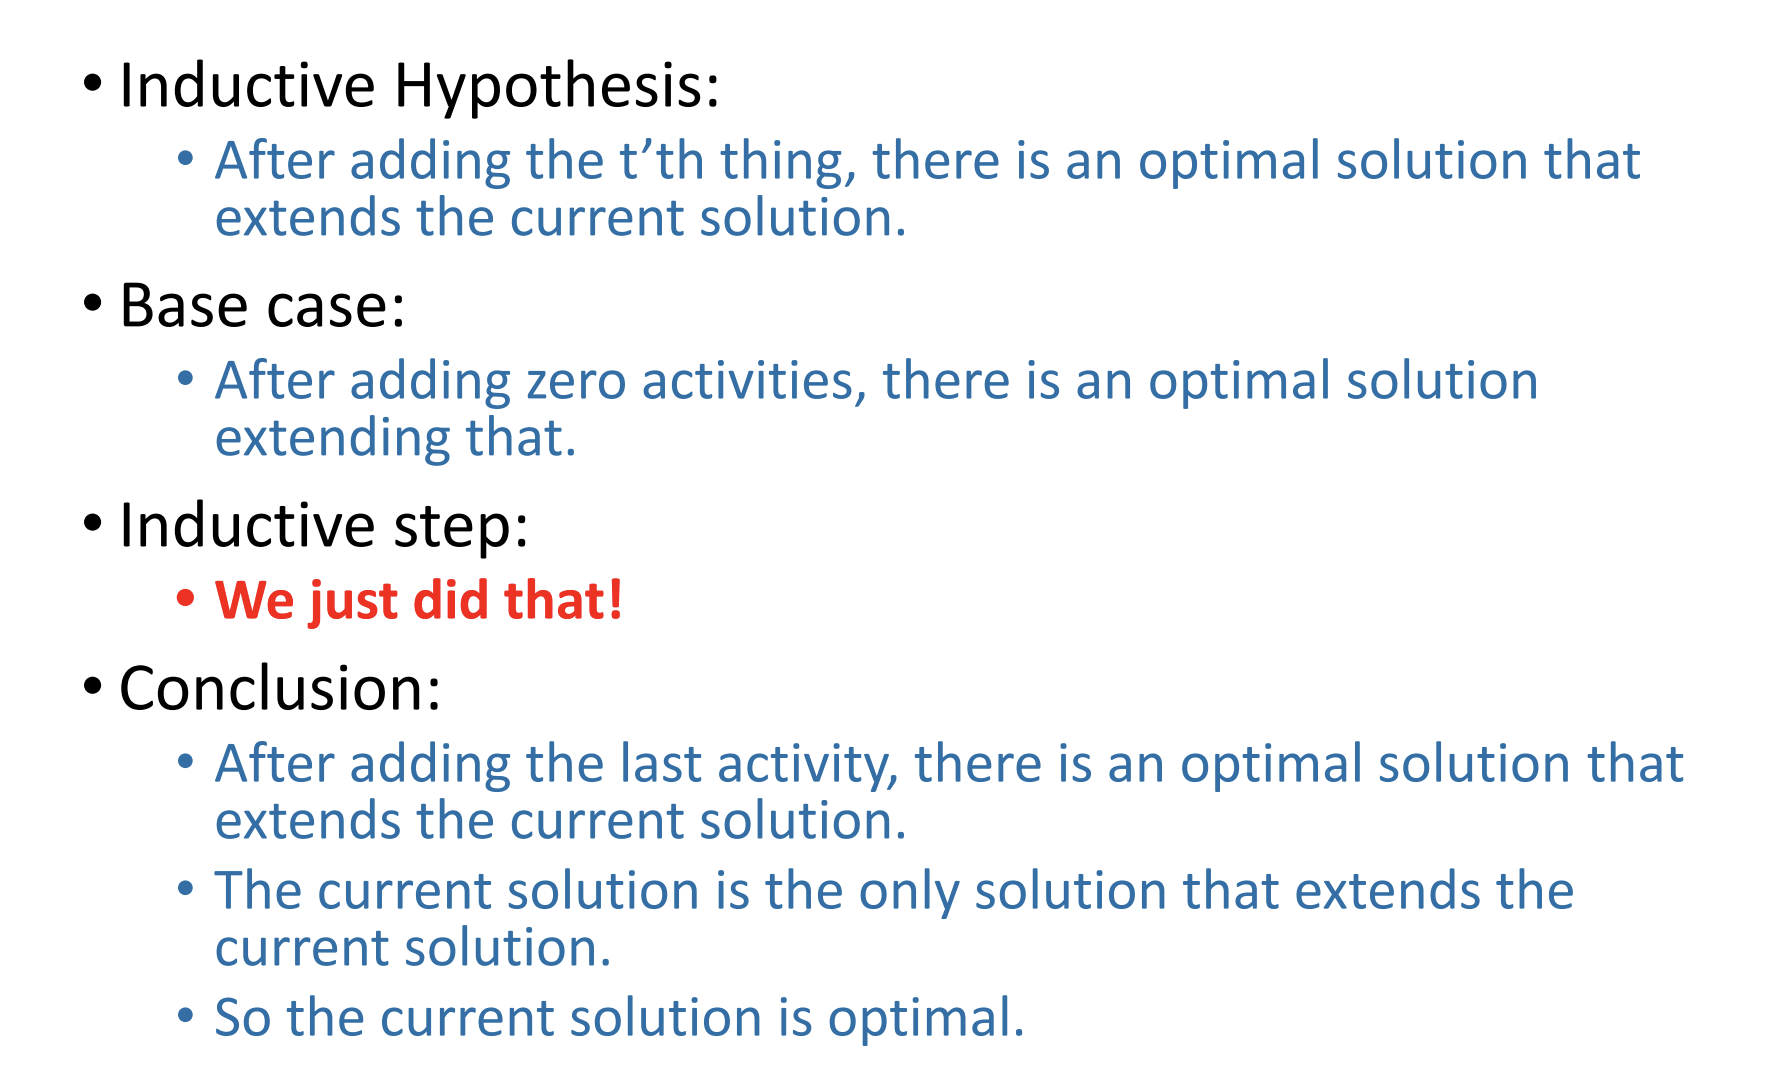
\includegraphics[scale=0.3]{greedyproof.png} 
\subsection*{Spanning trees}
\begin{itemize}
    \item a tree is just a connected graph with $n-1$ edges
    \item a spanning tree is some subgraph of the original that is still connected but has no cycles
\end{itemize}
\subsubsection*{Minimum spanning tree}
\begin{itemize}
    \item spanning tree with min. weight 
    \item i.e. what's the least amount of effort we need to connect everything together?
    \item why do we care? network design, cluster analysis, image processing
\end{itemize}

\subsubsection*{Prim's Algorithm}
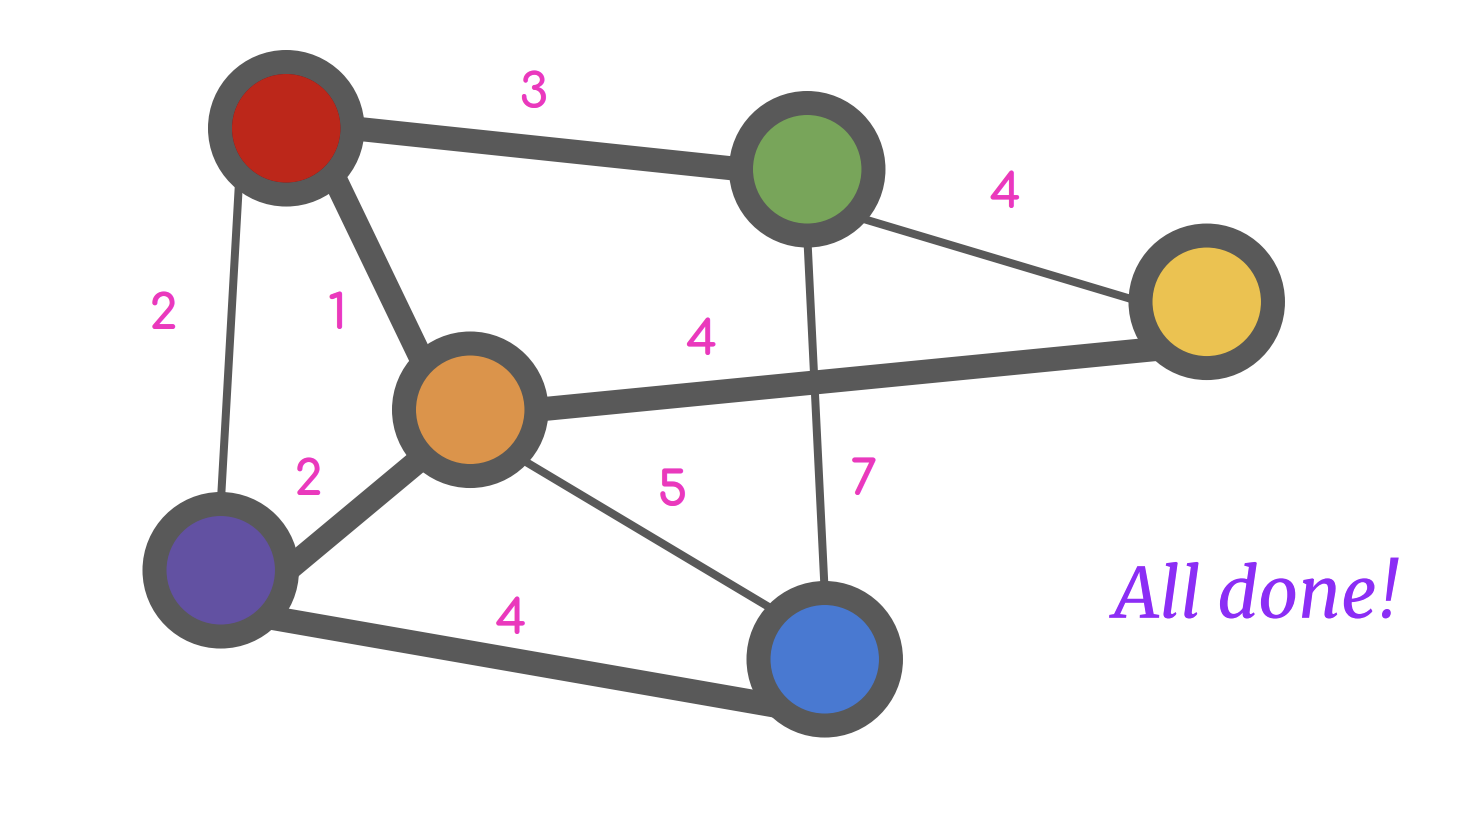
\includegraphics[scale=0.3]{prim.png} \\ 
Goal: Find MSTs. 
\\\\
Pseudocode: Repeat until all vertices are connected:
\begin{itemize}
    \item Choose an arbitrary starting vertex
    \item Find the lowest cost edge that would connect the current set of vertices to another vertex
\end{itemize}
Runtime: Uses a Fibonacci heap to run in $O(n \log n + m)$
time. Here, the heap is keeping track of which
vertex that we haven't used yet is closest
to some vertex we have used.
\subsection*{Ford-Fulkerson}
Goal: Find max flow in a graph.
\\\\
Pseudocode:
\begin{itemize}
    \item Start with zero flow
    \item We will maintain a “residual graph” $G_f$
    \item A path from s to t in $G_f$ will give us a way to improve our flow.
    \begin{itemize}
     \item Definition: A path from s to t in the residual network is called an \textbf{augmenting path}.
    \item Claim: If there is an augmenting path, we can increase the flow along that path
    \end{itemize}
    \item We will continue until there are no s-t paths left.
\end{itemize}
\end{document}

